\chapter{FLOATING POINT COMPRESSION}
\label{chp:fzip}
\newif\ifshort

%\shortfalse
%or
\shorttrue

\newif\ifbwtsec

\bwtsecfalse
%\bwtsectrue
Floating point compression is the second half of matrix compression. \figurename~\ref{tbl:value} shows a comparison of compression schemes. In the end, we created a program and library called fzip. In total, fzip takes advantage of 2 compressible features of datasets: repeating values (patterns exactly 8 bytes long), and repeating prefixes (patterns less than 8 bytes long). For SpMV, we need to make a hardware decoder. So taking advantage of sequences that are more than 8 bytes long is difficult. In the remainder of this chapter we talk about an analysis of floating point datasets (Section \ref{sec:fzipanalysis}), our approach to floating point compression (Section \ref{sec:fzipapproach}), our hardware decoder (Section~\ref{sec:fzip_decoder}) and our results (Section \ref{sec:fzipdiscussion}).

\begin{table*}
\centering
\begin{threeparttable}
    \caption[Value compression analysis.]{Detailed value compression analysis and performance comparison, in terms of bytes per non-zero value.}
\label{tbl:value}
\begin{tabular}{ccccccccc}
\hline
\bfseries Matrix & \bfseries \tikz \node[rotate=90]{uncompressed}; & \bfseries \tikz \node[rotate=90]{Unique Values}; & \bfseries \tikz \node[rotate=90]{Unique/nnz $\times 8$}; & \bfseries \tikz \node[rotate=90]{256 Common}; & \bfseries \tikz \node[rotate=90]{GZIP}; & \bfseries \tikz \node[rotate=90]{FPC};\\
\hline
dense2\tnote{a} & $8.00$ & $1.00$ & $0.00$ & $1.00$ & $0.01$ & $0.50$ \\
pdb1HYS & $8.00$ & $1.10 \times 10^{6}$ & $4.08$ & $7.99$ & $4.15$ & $7.99$  \\
consph & $8.00$ & $1.24 \times 10^{6}$ & $3.28$ & $7.99$ & $5.10$ & $7.95$  \\
cant & $8.00$ & $1.07 \times 10^{2}$ & $0.00$ & $1.00$ & $0.11$ & $0.91$  \\
pwtk & $8.00$ & $3.63 \times 10^{6}$ & $5.04$ & $7.95$ & $4.29$ & $7.37$  \\
rma10\tnote{a} & $8.00$ & $1.00$ & $0.00$ & $1.00$ & $0.01$ & $0.50$  \\
qcd5\_4\tnote{a} & $8.00$ & $1.00$ & $0.00$ & $1.00$ & $0.01$ & $0.50$  \\
shipsec1 & $8.00$ & $8.86 \times 10^{4}$ & $0.56$ & $6.39$ & $2.08$ & $3.80$ \\
mac\_econ\_fwd500 & $8.00$ & $1.08 \times 10^{5}$ & $1.36$ & $5.20$ & $0.73$ & $1.45$ \\
mc2depi & $8.00$ & $3.58 \times 10^{3}$ & $0.00$ & $4.94$ & $1.24$ & $5.01$ \\
cop20k\_A & $8.00$ & $9.56 \times 10^{5}$ & $5.84$ & $7.97$ & $5.53$ & $7.97$ \\
scircuit & $8.00$ & $8.82 \times 10^{4}$ & $1.44$ & $5.41$ & $1.95$ & $3.68$ \\
webbase-1M & $8.00$ & $5.65 \times 10^{2}$ & $0.00$ & $1.48$ & $0.38$ & $1.92$ \\
\hline
average\tnote{b} & $8.00$ & $7.22 \times 10^{5}$ & $2.16$ & $5.63$ & $2.56$ & $4.81$ \\

\hline
\end{tabular}
\begin{tablenotes}
\item [a] Boolean matrices
\item [b] Excludes boolean matrices
\end{tablenotes}
\end{threeparttable}
\end{table*}
%
\section{Related Work}
\label{sec:fziprelated}
It was noted in \cite{prelim:kourtis, prelim:grigoras} that sparse matrices often have repeated values. This is the focus of our value compression. Our previous work ($R^3$) had a simple scheme using this feature. It stored the 256 most common values so those common values could be represented as one byte. The performance of this scheme is shown in the column ``256 common" in Table~\ref{tbl:value}.\par
We analyze gzip, bzip and FPC [\cite{prelim:burtscher}] to see how high a compression ratio over the uncompressed 8 bytes per value is achievable.\par
Uncompressed data would take 8 bytes per element. Any good compression scheme should take less than 8 bytes per element. We looked at \cite{prelim:burtscher} describing its own compression scheme, FPC. This scheme looks for repeated patterns. However it does not exploit the fact most of its compression comes from exact (8 byte) value repeats. To illustrate this point we created an ``anti-FPC" dataset (\figurename~\ref{fig:antiFpc}).
\begin{figure}
    \center
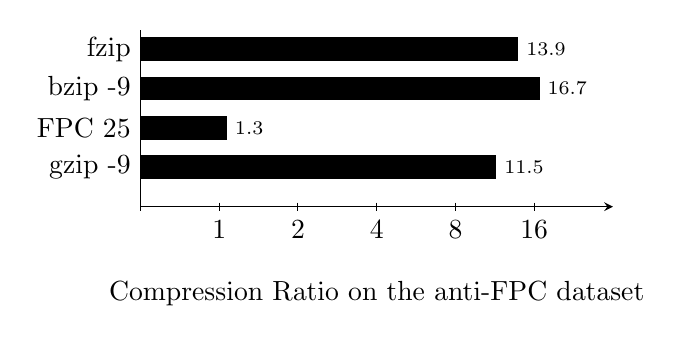
\begin{tikzpicture}[yscale=.5]
\draw (0,0) -- (0,4.5);
\draw[-stealth] (0,0) -- (6,0);
\foreach \x/\n in {0/,1/1,2/2,3/4,4/8,5/16}{
    \draw (\x,.1) -- (\x,-.1)node[anchor=north]{\n};
}
\node at (3,-2.2){Compression Ratio on the anti-FPC dataset};
\foreach \y/\n in {0/,1/gzip -9,2/FPC 25,3/bzip -9,4/fzip}{
    \node[anchor=east, rotate=0] at (0,\y){\n};
}
\scriptsize
\foreach \x/\y/\n in {4.52/1/11.5,1.1/2/1.3,5.07/3/16.7,4.8/4/13.9}{
    \fill (0,\y-.3) rectangle (\x,\y+.3);
    \node[anchor=west] at (\x,\y){\n};
}
\end{tikzpicture}
\caption[The Anti-FPC dataset]{We engineering a dataset to make the performance of FPC look bad compared to other programs. Although unfair, this shows a type of pattern that FPC does not exploit and other programs do. This problem exists because FPC only uses predictors for compression.}
\label{fig:antiFpc}
\end{figure}

\par gzip performs quite well too. We have a general understanding of how gzip works. We suspect the reason for the good performance is the large memory space and being able to look up previously occurring 8-byte values.
\par Our focus on using repeated values is reinforced by looking at the number of unique values. If only the unique values were stored the average compression would be $2.16$ bytes per element. This can not be used by itself since this ignores the indexing required to access these values, but this gives an estimate of the possible compression size.
\begin{figure}
\center
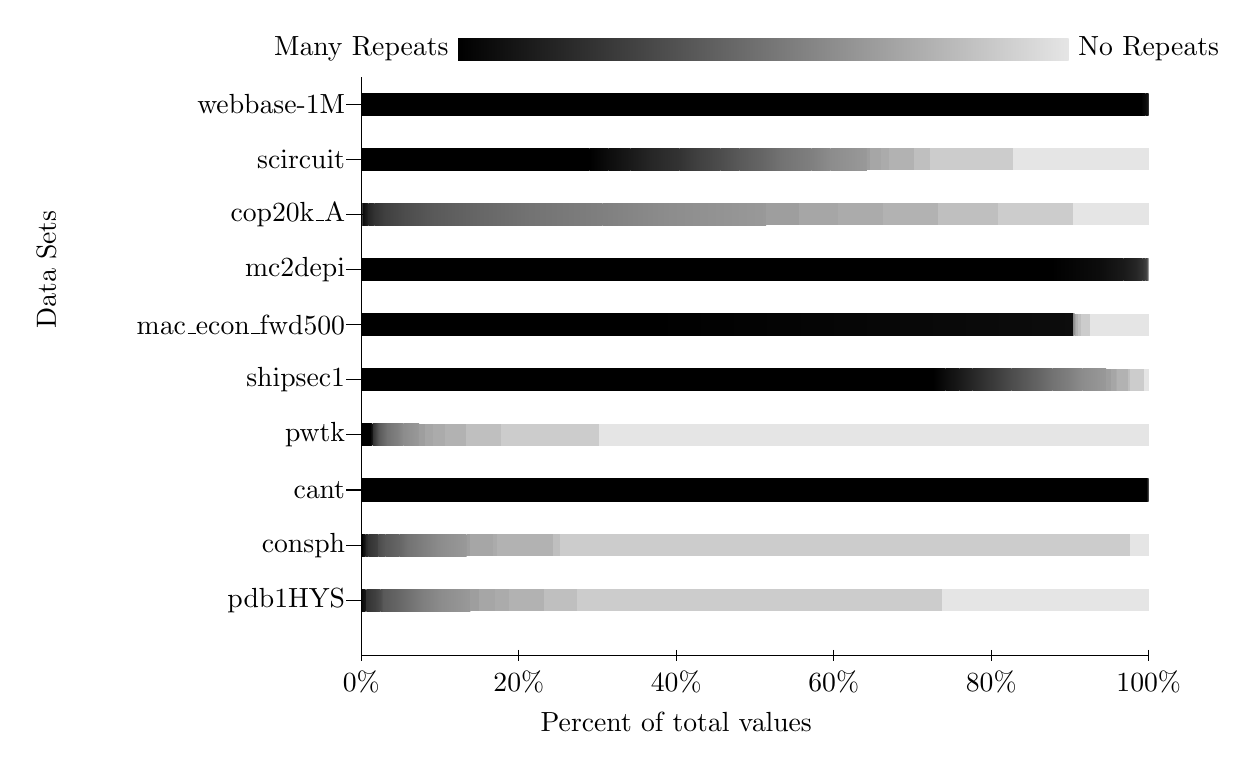
\begin{tikzpicture}[yscale=.7,xscale=2]

\path[draw] (0,0) -- (0,10.5);
\path[draw] (0,0) -- (5,0);
\foreach \x/\v in {0/0,1/20,2/40,3/60,4/80,5/100}{
    \draw (\x,.1) -- (\x,-.1)node[anchor=north]{\v\%};
}

\foreach \n/\y in {pdb1HYS/1, consph/2, cant/3, pwtk/4, shipsec1/5, mac\_econ\_fwd500/6, mc2depi/7, cop20k\_A/8, scircuit/9, webbase-1M/10}{
    \draw (.1,\y) -- (-.1,\y)node[anchor=east,rotate=0,inner sep=0]{\n};
}
\node at (2,-1.2){Percent of total values};
\node[rotate=90] at (-2,7){Data Sets};

%pdb1HYS
\foreach \xa/\xb/\sa/\sb in {0/0.00457/100/100,0.00457/0.00531/100/95,0.00531/0.0281/95/90,0.0281/0.0313/90/85,0.0313/0.0327/85/80,0.0327/0.0879/80/75,0.0879/0.123/75/70,0.123/0.139/70/65,0.139/0.234/65/60,0.234/0.314/60/55,0.314/0.398/55/50,0.398/0.507/50/45,0.507/0.692/45/40,}{
    \shade[left color=black!\sa,right color=black!\sb] (\xa,0.8) rectangle (\xb,1.2);
}
\foreach \xa/\xb/\s in {0.692/0.748/38,0.748/0.847/35,0.847/0.939/33,0.939/1.16/30,1.16/1.37/25,1.37/3.69/20,3.69/5/10}{
    \fill[black!\s] (\xa,0.8) rectangle (\xb,1.2);
}
%consph
\foreach \xa/\xb/\sa/\sb in {0/0.00387/100/100,0.00387/0.0118/100/95,0.0118/0.0268/95/90,0.0268/0.0274/90/85,0.0274/0.0464/85/80,0.0464/0.0992/80/75,0.0992/0.11/75/70,0.11/0.154/70/65,0.154/0.242/65/60,0.242/0.295/60/55,0.295/0.398/55/50,0.398/0.5/50/45,0.5/0.668/45/40,}{
    \shade[left color=black!\sa,right color=black!\sb] (\xa,1.8) rectangle (\xb,2.2);
}
\foreach \xa/\xb/\s in {0.668/0.689/38,0.689/0.834/35,0.834/0.86/33,0.86/1.22/30,1.22/1.26/25,1.26/4.88/20,4.88/5/10}{
    \fill[black!\s] (\xa,1.8) rectangle (\xb,2.2);
}
%cant
\foreach \xa/\xb/\sa/\sb in {0/4.99/100/100,4.99/4.99/100/95,4.99/4.99/95/90,4.99/5/90/85,5/5/85/80,5/5/80/75,5/5/75/70,5/5/70/65,5/5/65/60,5/5/60/55,5/5/55/50,5/5/50/45,}{
    \shade[left color=black!\sa,right color=black!\sb] (\xa,2.8) rectangle (\xb,3.2);
}
\foreach \xa/\xb/\s in {5/5/38,5/5/10}{
    \fill[black!\s] (\xa,2.8) rectangle (\xb,3.2);
}
%pwtk
\foreach \xa/\xb/\sa/\sb in {0/0.0608/100/100,0.0608/0.0628/100/95,0.0628/0.0705/95/90,0.0705/0.0729/90/85,0.0729/0.0751/85/80,0.0751/0.0873/80/75,0.0873/0.0988/75/70,0.0988/0.111/70/65,0.111/0.138/65/60,0.138/0.164/60/55,0.164/0.227/55/50,0.227/0.268/50/45,0.268/0.367/45/40,}{
    \shade[left color=black!\sa,right color=black!\sb] (\xa,3.8) rectangle (\xb,4.2);
}
\foreach \xa/\xb/\s in {0.367/0.402/38,0.402/0.458/35,0.458/0.529/33,0.529/0.667/30,0.667/0.884/25,0.884/1.51/20,1.51/5/10}{
    \fill[black!\s] (\xa,3.8) rectangle (\xb,4.2);
}
%shipsec1
\foreach \xa/\xb/\sa/\sb in {0/3.63/100/100,3.63/3.71/100/95,3.71/3.8/95/90,3.8/3.88/90/85,3.88/3.96/85/80,3.96/4.05/80/75,4.05/4.13/75/70,4.13/4.22/70/65,4.22/4.31/65/60,4.31/4.39/60/55,4.39/4.5/55/50,4.5/4.58/50/45,4.58/4.73/45/40,}{
    \shade[left color=black!\sa,right color=black!\sb] (\xa,4.8) rectangle (\xb,5.2);
}
\foreach \xa/\xb/\s in {4.73/4.76/38,4.76/4.79/35,4.79/4.8/33,4.8/4.87/30,4.87/4.88/25,4.88/4.97/20,4.97/5/10}{
    \fill[black!\s] (\xa,4.8) rectangle (\xb,5.2);
}
%mac_econ_fwd500
\foreach \xa/\xb/\sa/\sb in {0/1.84/100/100,1.84/4.52/100/95,4.52/4.52/95/90,4.52/4.52/90/85,4.52/4.52/85/80,4.52/4.52/80/75,4.52/4.52/75/70,4.52/4.52/70/65,4.52/4.52/65/60,4.52/4.52/60/55,4.52/4.52/55/50,4.52/4.52/50/45,4.52/4.53/45/40,}{
    \shade[left color=black!\sa,right color=black!\sb] (\xa,5.8) rectangle (\xb,6.2);
}
\foreach \xa/\xb/\s in {4.53/4.53/38,4.53/4.54/35,4.54/4.54/33,4.54/4.55/30,4.55/4.57/25,4.57/4.63/20,4.63/5/10}{
    \fill[black!\s] (\xa,5.8) rectangle (\xb,6.2);
}
%mc2depi
\foreach \xa/\xb/\sa/\sb in {0/4.38/100/100,4.38/4.69/100/95,4.69/4.84/95/90,4.84/4.92/90/85,4.92/4.96/85/80,4.96/4.98/80/75,4.98/4.99/75/70,4.99/4.99/70/65,4.99/5/65/60,5/5/60/55,5/5/55/50,5/5/50/45,5/5/45/40,}{
    \shade[left color=black!\sa,right color=black!\sb] (\xa,6.8) rectangle (\xb,7.2);
}
\foreach \xa/\xb/\s in {5/5/38,5/5/35,5/5/33,5/5/30,5/5/25,5/5/20,5/5/10}{
    \fill[black!\s] (\xa,6.8) rectangle (\xb,7.2);
}
%cop20k_A
\foreach \xa/\xb/\sa/\sb in {0/0.00668/100/100,0.00668/0.0122/100/95,0.0122/0.0298/95/90,0.0298/0.0471/90/85,0.0471/0.0842/85/80,0.0842/0.149/80/75,0.149/0.277/75/70,0.277/0.455/70/65,0.455/0.74/65/60,0.74/1.07/60/55,1.07/1.53/55/50,1.53/1.94/50/45,1.94/2.57/45/40,}{
    \shade[left color=black!\sa,right color=black!\sb] (\xa,7.8) rectangle (\xb,8.2);
}
\foreach \xa/\xb/\s in {2.57/2.78/38,2.78/3.03/35,3.03/3.31/33,3.31/3.66/30,3.66/4.04/25,4.04/4.52/20,4.52/5/10}{
    \fill[black!\s] (\xa,7.8) rectangle (\xb,8.2);
}
%scircuit
\foreach \xa/\xb/\sa/\sb in {0/1.45/100/100,1.45/1.57/100/95,1.57/1.71/95/90,1.71/1.84/90/85,1.84/2.02/85/80,2.02/2.13/80/75,2.13/2.28/75/70,2.28/2.4/70/65,2.4/2.55/65/60,2.55/2.67/60/55,2.67/2.86/55/50,2.86/2.98/50/45,2.98/3.21/45/40,}{
    \shade[left color=black!\sa,right color=black!\sb] (\xa,8.8) rectangle (\xb,9.2);
}
\foreach \xa/\xb/\s in {3.21/3.23/38,3.23/3.3/35,3.3/3.35/33,3.35/3.51/30,3.51/3.61/25,3.61/4.14/20,4.14/5/10}{
    \fill[black!\s] (\xa,8.8) rectangle (\xb,9.2);
}
%webbase-1M
\foreach \xa/\xb/\sa/\sb in {0/4.95/100/100,4.95/4.98/100/95,4.98/5/95/90,}{
    \shade[left color=black!\sa,right color=black!\sb] (\xa,9.8) rectangle (\xb,10.2);
}
\foreach \xa/\xb/\s in {5/5/89,5/5/10}{
    \fill[black!\s] (\xa,9.8) rectangle (\xb,10.2);
}

%key
\node[fill=white] at (0,11)(high){Many Repeats};
\node[fill=white] at (5,11)(low){No Repeats};
\shade[left color=black,right color=black!10] ([yshift=-.2cm]high.east) rectangle ([yshift=.2cm]low.west);

\end{tikzpicture}
\caption[Floating point repeat analysis.]{The above figure shows the distribution of repeats in each dataset. Each shade represents a different number of repeats. For instance: \tikz \fill (0,0) rectangle (.2,.2);:$>512$, \tikz \fill[black!50] (0,0) rectangle (.2,.2);:$16$, \tikz \fill[black!20] (0,0) rectangle (.2,.2);:$2$, \tikz \fill[black!10] (0,0) rectangle (.2,.2);:$1$(no repeats).}
\label{fig:repeat}
\end{figure}

\section{Floating-Point Value Analysis}
\label{sec:fzipanalysis}
Continuing the analysis from the beginning of this chapter, \figurename~\ref{fig:repeat} shows an analysis of the repeating values in each of the datasets used for testing. Several characteristics of this analysis suggest that compressing repeating values will perform well. For example, in more than half of the datasets at least 80\% of the values repeat.\\
\indent
Another pattern exists among the prefixes of the values. To understand why, look at the floating point data structure. Double-precision floating-point values have 3 parts: a sign bit, 11 exponent bits and 52 fraction bits. Values close to each other in the dataset often share the same sign. (Some datasets only contain positive numbers.) Likewise, close values often share the most significant bits of the exponent. In fact, the bits in floating-point values already exist in most likely shared to least likely shared sorted order: \{sign bit, most significant exponent bits, least significant exponent bits, most significant fraction bits, least significant fraction bits\}.\\
\indent We gauge the strength of the pattern in a particular dataset by looking at how many prefix bits the adjacent values share. \figurename~\ref{fig:prefix} describes this analysis. From this figure, we see that the first byte or so often repeats. However, there usually exists a rapid decline in shared bits after this point.\par
\begin{figure}
\center
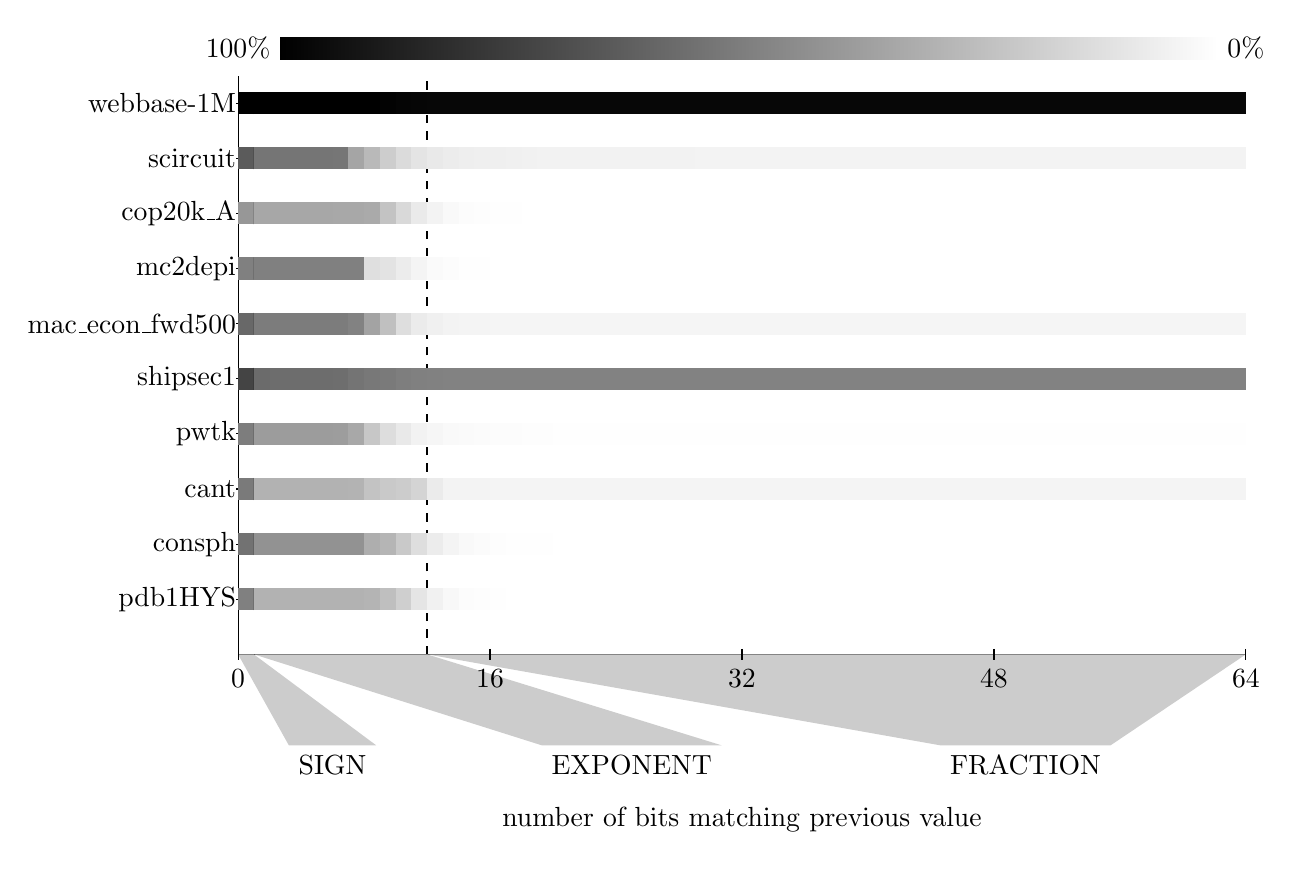
\begin{tikzpicture}[xscale=.2, yscale=.7]
\path[draw] (0,0) -- (64,0);
\path[draw] (0,0) -- (0, 10.5);
\path[draw,dashed] (12,0) -- (12,10.5);
\node(sign) at (6,-2){SIGN};
\node(expo) at (25,-2){EXPONENT};
\node(frac) at (50,-2){FRACTION};
\path[fill=black!20](0,0) -- (1,0) -- (sign.north east) -- (sign.north west) -- cycle;
\path[fill=black!20](1,0) -- (12,0) -- (expo.north east) -- (expo.north west) -- cycle;
\path[fill=black!20](12,0) -- (64,0) -- (frac.north east) -- (frac.north west) -- cycle;

\node[fill=white] at (0,11)(high){100\%};
\node[fill=white] at (64,11)(low){0\%};
\shade[left color=black,right color=white] ([yshift=-.2cm]high.east) rectangle ([yshift=.2cm]low.west);
\foreach \x in {0,16,32,48,64}{
    \draw (\x,.1) -- (\x,-.1)node[anchor=north]{\x};
}

\foreach \n/\y in {pdb1HYS/1, consph/2, cant/3, pwtk/4, shipsec1/5, mac\_econ\_fwd500/6, mc2depi/7, cop20k\_A/8, scircuit/9, webbase-1M/10}{
    \draw (.1,\y) -- (-.1,\y)node[anchor=east,rotate=0,inner sep=0]{\n};
}
\node at (32,-3) {number of bits matching previous value};

    %\shade[left color=black!\ya, right color=black!\yb] (\xa,0.8) rectangle (\xb,1.2);
    %\fill[color=black!\yb] (\xa,0.8) rectangle (\xb,1.2);
\foreach \xa/\ya/\xb/\yb in {
0/100.00/1/49.85,1/49.85/2/30.14,2/30.14/3/30.14,3/30.14/4/30.14,4/30.14/5/30.14,5/30.14/6/30.14,6/30.14/7/30.14,7/30.14/8/30.09,8/30.09/9/29.23,9/29.23/10/25.06,10/25.06/11/18.88,11/18.88/12/10.34,12/10.34/13/5.36,13/5.36/14/2.62,14/2.62/15/1.31,15/1.31/16/0.66,16/0.66/17/0.33,17/0.33/18/0.16,18/0.16/19/0.08,19/0.08/20/0.04,20/0.04/21/0.02,21/0.02/22/0.01,22/0.01/23/0.01,23/0.01/24/0.01,24/0.01/25/0.01,25/0.01/26/0.01,26/0.01/27/0.01,27/0.01/28/0.01,28/0.01/29/0.01,29/0.01/30/0.01,30/0.01/31/0.01,31/0.01/32/0.01,32/0.01/33/0.01,33/0.01/34/0.01,34/0.01/35/0.01,35/0.01/36/0.01,36/0.01/37/0.01,37/0.01/38/0.01,38/0.01/39/0.01,39/0.01/40/0.01,40/0.01/41/0.01,41/0.01/42/0.01,42/0.01/43/0.01,43/0.01/44/0.01,44/0.01/45/0.01,45/0.01/46/0.01,46/0.01/47/0.01,47/0.01/48/0.01,48/0.01/49/0.01,49/0.01/50/0.01,50/0.01/51/0.01,51/0.01/52/0.01,52/0.01/53/0.01,53/0.01/54/0.01,54/0.01/55/0.01,55/0.01/56/0.01,56/0.01/57/0.01,57/0.01/58/0.01,58/0.01/59/0.01,59/0.01/60/0.01,60/0.01/61/0.01,61/0.01/62/0.01,62/0.01/63/0.01,63/0.01/64/0.01,}{
    \fill[color=black!\yb] (\xa,0.8) rectangle (\xb,1.2);
}
\foreach \xa/\ya/\xb/\yb in {
0/100.00/1/55.40,1/55.40/2/42.65,2/42.65/3/42.65,3/42.65/4/42.65,4/42.65/5/42.65,5/42.65/6/42.65,6/42.65/7/42.65,7/42.65/8/42.64,8/42.64/9/31.79,9/31.79/10/28.98,10/28.98/11/21.30,11/21.30/12/12.99,12/12.99/13/7.55,13/7.55/14/4.33,14/4.33/15/2.49,15/2.49/16/1.43,16/1.43/17/0.83,17/0.83/18/0.51,18/0.51/19/0.33,19/0.33/20/0.24,20/0.24/21/0.19,21/0.19/22/0.16,22/0.16/23/0.15,23/0.15/24/0.14,24/0.14/25/0.14,25/0.14/26/0.14,26/0.14/27/0.14,27/0.14/28/0.14,28/0.14/29/0.13,29/0.13/30/0.13,30/0.13/31/0.13,31/0.13/32/0.13,32/0.13/33/0.13,33/0.13/34/0.13,34/0.13/35/0.13,35/0.13/36/0.13,36/0.13/37/0.13,37/0.13/38/0.13,38/0.13/39/0.13,39/0.13/40/0.13,40/0.13/41/0.13,41/0.13/42/0.13,42/0.13/43/0.13,43/0.13/44/0.13,44/0.13/45/0.13,45/0.13/46/0.13,46/0.13/47/0.13,47/0.13/48/0.13,48/0.13/49/0.13,49/0.13/50/0.13,50/0.13/51/0.13,51/0.13/52/0.13,52/0.13/53/0.13,53/0.13/54/0.13,54/0.13/55/0.13,55/0.13/56/0.13,56/0.13/57/0.13,57/0.13/58/0.13,58/0.13/59/0.13,59/0.13/60/0.13,60/0.13/61/0.13,61/0.13/62/0.13,62/0.13/63/0.13,63/0.13/64/0.13,}{
    \fill[color=black!\yb] (\xa,1.8) rectangle (\xb,2.2);
}
\foreach \xa/\ya/\xb/\yb in {
0/100.00/1/52.33,1/52.33/2/30.36,2/30.36/3/30.36,3/30.36/4/30.36,4/30.36/5/30.36,5/30.36/6/30.36,6/30.36/7/30.13,7/30.13/8/29.96,8/29.96/9/23.37,9/23.37/10/21.31,10/21.31/11/19.95,11/19.95/12/17.04,12/17.04/13/7.94,13/7.94/14/4.56,14/4.56/15/4.56,15/4.56/16/4.53,16/4.53/17/4.37,17/4.37/18/4.36,18/4.36/19/4.36,19/4.36/20/4.35,20/4.35/21/4.35,21/4.35/22/4.35,22/4.35/23/4.35,23/4.35/24/4.35,24/4.35/25/4.35,25/4.35/26/4.35,26/4.35/27/4.35,27/4.35/28/4.35,28/4.35/29/4.35,29/4.35/30/4.35,30/4.35/31/4.35,31/4.35/32/4.35,32/4.35/33/4.35,33/4.35/34/4.35,34/4.35/35/4.35,35/4.35/36/4.35,36/4.35/37/4.35,37/4.35/38/4.35,38/4.35/39/4.35,39/4.35/40/4.35,40/4.35/41/4.35,41/4.35/42/4.35,42/4.35/43/4.35,43/4.35/44/4.35,44/4.35/45/4.35,45/4.35/46/4.35,46/4.35/47/4.35,47/4.35/48/4.35,48/4.35/49/4.35,49/4.35/50/4.35,50/4.35/51/4.35,51/4.35/52/4.35,52/4.35/53/4.35,53/4.35/54/4.35,54/4.35/55/4.35,55/4.35/56/4.35,56/4.35/57/4.35,57/4.35/58/4.35,58/4.35/59/4.35,59/4.35/60/4.35,60/4.35/61/4.35,61/4.35/62/4.35,62/4.35/63/4.35,63/4.35/64/4.35,}{
    \fill[color=black!\yb] (\xa,2.8) rectangle (\xb,3.2);
}
\foreach \xa/\ya/\xb/\yb in {
0/100.00/1/50.92,1/50.92/2/38.78,2/38.78/3/38.68,3/38.68/4/38.68,4/38.68/5/38.68,5/38.68/6/38.68,6/38.68/7/38.62,7/38.62/8/33.96,8/33.96/9/22.15,9/22.15/10/13.32,10/13.32/11/8.67,11/8.67/12/5.24,12/5.24/13/3.42,13/3.42/14/2.37,14/2.37/15/1.87,15/1.87/16/1.55,16/1.55/17/1.33,17/1.33/18/1.06,18/1.06/19/0.80,19/0.80/20/0.63,20/0.63/21/0.49,21/0.49/22/0.44,22/0.44/23/0.43,23/0.43/24/0.42,24/0.42/25/0.41,25/0.41/26/0.41,26/0.41/27/0.41,27/0.41/28/0.41,28/0.41/29/0.41,29/0.41/30/0.41,30/0.41/31/0.41,31/0.41/32/0.41,32/0.41/33/0.41,33/0.41/34/0.41,34/0.41/35/0.41,35/0.41/36/0.41,36/0.41/37/0.41,37/0.41/38/0.41,38/0.41/39/0.41,39/0.41/40/0.41,40/0.41/41/0.41,41/0.41/42/0.41,42/0.41/43/0.41,43/0.41/44/0.41,44/0.41/45/0.41,45/0.41/46/0.41,46/0.41/47/0.41,47/0.41/48/0.41,48/0.41/49/0.41,49/0.41/50/0.41,50/0.41/51/0.41,51/0.41/52/0.41,52/0.41/53/0.41,53/0.41/54/0.41,54/0.41/55/0.41,55/0.41/56/0.41,56/0.41/57/0.41,57/0.41/58/0.41,58/0.41/59/0.41,59/0.41/60/0.41,60/0.41/61/0.41,61/0.41/62/0.41,62/0.41/63/0.41,63/0.41/64/0.41,}{
    \fill[color=black!\yb] (\xa,3.8) rectangle (\xb,4.2);
}
\foreach \xa/\ya/\xb/\yb in {
0/100.00/1/73.19,1/73.19/2/58.16,2/58.16/3/57.23,3/57.23/4/57.23,4/57.23/5/57.23,5/57.23/6/57.23,6/57.23/7/56.76,7/56.76/8/54.57,8/54.57/9/52.94,9/52.94/10/52.02,10/52.02/11/50.78,11/50.78/12/49.92,12/49.92/13/49.38,13/49.38/14/49.14,14/49.14/15/49.03,15/49.03/16/48.99,16/48.99/17/48.98,17/48.98/18/48.96,18/48.96/19/48.96,19/48.96/20/48.96,20/48.96/21/48.96,21/48.96/22/48.95,22/48.95/23/48.95,23/48.95/24/48.95,24/48.95/25/48.95,25/48.95/26/48.95,26/48.95/27/48.95,27/48.95/28/48.95,28/48.95/29/48.95,29/48.95/30/48.95,30/48.95/31/48.95,31/48.95/32/48.95,32/48.95/33/48.95,33/48.95/34/48.95,34/48.95/35/48.95,35/48.95/36/48.95,36/48.95/37/48.95,37/48.95/38/48.95,38/48.95/39/48.95,39/48.95/40/48.95,40/48.95/41/48.95,41/48.95/42/48.95,42/48.95/43/48.95,43/48.95/44/48.95,44/48.95/45/48.95,45/48.95/46/48.95,46/48.95/47/48.95,47/48.95/48/48.95,48/48.95/49/48.95,49/48.95/50/48.95,50/48.95/51/48.95,51/48.95/52/48.95,52/48.95/53/48.95,53/48.95/54/48.95,54/48.95/55/48.95,55/48.95/56/48.95,56/48.95/57/48.95,57/48.95/58/48.95,58/48.95/59/48.95,59/48.95/60/48.95,60/48.95/61/48.95,61/48.95/62/48.95,62/48.95/63/48.95,63/48.95/64/48.95,}{
    \fill[color=black!\yb] (\xa,4.8) rectangle (\xb,5.2);
}
\foreach \xa/\ya/\xb/\yb in {
0/100.00/1/59.09,1/59.09/2/51.55,2/51.55/3/51.55,3/51.55/4/51.55,4/51.55/5/51.55,5/51.55/6/51.55,6/51.55/7/51.55,7/51.55/8/48.90,8/48.90/9/35.89,9/35.89/10/24.78,10/24.78/11/12.76,11/12.76/12/7.66,12/7.66/13/5.82,13/5.82/14/4.89,14/4.89/15/4.46,15/4.46/16/4.21,16/4.21/17/4.07,17/4.07/18/3.87,18/3.87/19/3.79,19/3.79/20/3.78,20/3.78/21/3.78,21/3.78/22/3.77,22/3.77/23/3.77,23/3.77/24/3.77,24/3.77/25/3.77,25/3.77/26/3.77,26/3.77/27/3.77,27/3.77/28/3.77,28/3.77/29/3.77,29/3.77/30/3.77,30/3.77/31/3.74,31/3.74/32/3.73,32/3.73/33/3.73,33/3.73/34/3.73,34/3.73/35/3.73,35/3.73/36/3.73,36/3.73/37/3.73,37/3.73/38/3.73,38/3.73/39/3.73,39/3.73/40/3.73,40/3.73/41/3.73,41/3.73/42/3.73,42/3.73/43/3.73,43/3.73/44/3.73,44/3.73/45/3.73,45/3.73/46/3.73,46/3.73/47/3.73,47/3.73/48/3.73,48/3.73/49/3.73,49/3.73/50/3.73,50/3.73/51/3.73,51/3.73/52/3.73,52/3.73/53/3.73,53/3.73/54/3.73,54/3.73/55/3.73,55/3.73/56/3.73,56/3.73/57/3.73,57/3.73/58/3.73,58/3.73/59/3.73,59/3.73/60/3.73,60/3.73/61/3.73,61/3.73/62/3.73,62/3.73/63/3.73,63/3.73/64/3.73,}{
    \fill[color=black!\yb] (\xa,5.8) rectangle (\xb,6.2);
}
\foreach \xa/\ya/\xb/\yb in {
0/100.00/1/49.93,1/49.93/2/49.85,2/49.85/3/49.85,3/49.85/4/49.85,4/49.85/5/49.85,5/49.85/6/49.85,6/49.85/7/49.85,7/49.85/8/49.85,8/49.85/9/12.48,9/12.48/10/11.11,10/11.11/11/7.59,11/7.59/12/4.18,12/4.18/13/2.09,13/2.09/14/1.05,14/1.05/15/0.52,15/0.52/16/0.26,16/0.26/17/0.13,17/0.13/18/0.07,18/0.07/19/0.04,19/0.04/20/0.02,20/0.02/21/0.02,21/0.02/22/0.02,22/0.02/23/0.02,23/0.02/24/0.02,24/0.02/25/0.02,25/0.02/26/0.02,26/0.02/27/0.02,27/0.02/28/0.02,28/0.02/29/0.02,29/0.02/30/0.02,30/0.02/31/0.02,31/0.02/32/0.02,32/0.02/33/0.02,33/0.02/34/0.02,34/0.02/35/0.02,35/0.02/36/0.02,36/0.02/37/0.02,37/0.02/38/0.02,38/0.02/39/0.02,39/0.02/40/0.02,40/0.02/41/0.02,41/0.02/42/0.02,42/0.02/43/0.02,43/0.02/44/0.02,44/0.02/45/0.02,45/0.02/46/0.02,46/0.02/47/0.02,47/0.02/48/0.02,48/0.02/49/0.02,49/0.02/50/0.02,50/0.02/51/0.02,51/0.02/52/0.02,52/0.02/53/0.02,53/0.02/54/0.02,54/0.02/55/0.02,55/0.02/56/0.02,56/0.02/57/0.02,57/0.02/58/0.02,58/0.02/59/0.02,59/0.02/60/0.02,60/0.02/61/0.02,61/0.02/62/0.02,62/0.02/63/0.02,63/0.02/64/0.02,}{
    \fill[color=black!\yb] (\xa,6.8) rectangle (\xb,7.2);
}
\foreach \xa/\ya/\xb/\yb in {
0/100.00/1/40.96,1/40.96/2/34.32,2/34.32/3/34.32,3/34.32/4/34.32,4/34.32/5/34.32,5/34.32/6/34.32,6/34.32/7/34.29,7/34.29/8/34.27,8/34.27/9/33.30,9/33.30/10/23.61,10/23.61/11/14.84,11/14.84/12/8.33,12/8.33/13/4.60,13/4.60/14/2.43,14/2.43/15/1.29,15/1.29/16/0.70,16/0.70/17/0.40,17/0.40/18/0.24,18/0.24/19/0.15,19/0.15/20/0.10,20/0.10/21/0.06,21/0.06/22/0.04,22/0.04/23/0.04,23/0.04/24/0.03,24/0.03/25/0.03,25/0.03/26/0.03,26/0.03/27/0.03,27/0.03/28/0.03,28/0.03/29/0.03,29/0.03/30/0.03,30/0.03/31/0.02,31/0.02/32/0.02,32/0.02/33/0.02,33/0.02/34/0.02,34/0.02/35/0.02,35/0.02/36/0.02,36/0.02/37/0.02,37/0.02/38/0.02,38/0.02/39/0.02,39/0.02/40/0.02,40/0.02/41/0.02,41/0.02/42/0.02,42/0.02/43/0.02,43/0.02/44/0.02,44/0.02/45/0.02,45/0.02/46/0.02,46/0.02/47/0.02,47/0.02/48/0.02,48/0.02/49/0.02,49/0.02/50/0.02,50/0.02/51/0.02,51/0.02/52/0.02,52/0.02/53/0.02,53/0.02/54/0.02,54/0.02/55/0.02,55/0.02/56/0.02,56/0.02/57/0.02,57/0.02/58/0.02,58/0.02/59/0.02,59/0.02/60/0.02,60/0.02/61/0.02,61/0.02/62/0.02,62/0.02/63/0.02,63/0.02/64/0.02,}{
    \fill[color=black!\yb] (\xa,7.8) rectangle (\xb,8.2);
}
\foreach \xa/\ya/\xb/\yb in {
0/100.00/1/64.34,1/64.34/2/54.22,2/54.22/3/54.22,3/54.22/4/54.22,4/54.22/5/54.22,5/54.22/6/54.22,6/54.22/7/53.67,7/53.67/8/35.26,8/35.26/9/27.48,9/27.48/10/19.55,10/19.55/11/14.08,11/14.08/12/10.56,12/10.56/13/8.73,13/8.73/14/7.60,14/7.60/15/6.81,15/6.81/16/6.44,16/6.44/17/6.11,17/6.11/18/5.91,18/5.91/19/5.51,19/5.51/20/5.29,20/5.29/21/5.24,21/5.24/22/5.09,22/5.09/23/5.07,23/5.07/24/5.04,24/5.04/25/4.99,25/4.99/26/4.97,26/4.97/27/4.93,27/4.93/28/4.92,28/4.92/29/4.91,29/4.91/30/4.90,30/4.90/31/4.90,31/4.90/32/4.90,32/4.90/33/4.90,33/4.90/34/4.90,34/4.90/35/4.89,35/4.89/36/4.89,36/4.89/37/4.88,37/4.88/38/4.87,38/4.87/39/4.87,39/4.87/40/4.87,40/4.87/41/4.87,41/4.87/42/4.87,42/4.87/43/4.87,43/4.87/44/4.87,44/4.87/45/4.87,45/4.87/46/4.87,46/4.87/47/4.87,47/4.87/48/4.87,48/4.87/49/4.87,49/4.87/50/4.87,50/4.87/51/4.87,51/4.87/52/4.87,52/4.87/53/4.87,53/4.87/54/4.87,54/4.87/55/4.87,55/4.87/56/4.87,56/4.87/57/4.87,57/4.87/58/4.87,58/4.87/59/4.87,59/4.87/60/4.87,60/4.87/61/4.87,61/4.87/62/4.87,62/4.87/63/4.87,63/4.87/64/4.87,}{
    \fill[color=black!\yb] (\xa,8.8) rectangle (\xb,9.2);
}
\foreach \xa/\ya/\xb/\yb in {
0/100.00/1/100.00,1/100.00/2/100.00,2/100.00/3/100.00,3/100.00/4/100.00,4/100.00/5/100.00,5/100.00/6/100.00,6/100.00/7/100.00,7/100.00/8/100.00,8/100.00/9/99.93,9/99.93/10/98.70,10/98.70/11/97.98,11/97.98/12/97.60,12/97.60/13/97.44,13/97.44/14/97.30,14/97.30/15/97.22,15/97.22/16/97.18,16/97.18/17/97.16,17/97.16/18/97.16,18/97.16/19/97.16,19/97.16/20/97.16,20/97.16/21/97.16,21/97.16/22/97.16,22/97.16/23/97.16,23/97.16/24/97.16,24/97.16/25/97.16,25/97.16/26/97.16,26/97.16/27/97.16,27/97.16/28/97.16,28/97.16/29/97.16,29/97.16/30/97.16,30/97.16/31/97.16,31/97.16/32/97.16,32/97.16/33/97.16,33/97.16/34/97.16,34/97.16/35/97.16,35/97.16/36/97.16,36/97.16/37/97.16,37/97.16/38/97.16,38/97.16/39/97.16,39/97.16/40/97.16,40/97.16/41/97.16,41/97.16/42/97.16,42/97.16/43/97.16,43/97.16/44/97.16,44/97.16/45/97.16,45/97.16/46/97.16,46/97.16/47/97.16,47/97.16/48/97.16,48/97.16/49/97.16,49/97.16/50/97.16,50/97.16/51/97.16,51/97.16/52/97.16,52/97.16/53/97.16,53/97.16/54/97.16,54/97.16/55/97.16,55/97.16/56/97.16,56/97.16/57/97.16,57/97.16/58/97.16,58/97.16/59/97.16,59/97.16/60/97.16,60/97.16/61/97.16,61/97.16/62/97.16,62/97.16/63/97.16,63/97.16/64/97.16,}{
    \fill[color=black!\yb] (\xa,9.8) rectangle (\xb,10.2);
}

\end{tikzpicture}
\caption[Floating point prefix analysis.]{The above figure represents local prefix prediction. The figure shows the density function of 2 adjacent values sharing at least $x$ number of prefix bits. All of the data sets start at $(0,100\%)$. The curves end at the percent of values that are identical to their previous value for that dataset.}
\label{fig:prefix}
\end{figure}%
Datasets might also have repeating patterns of values. For example, the sequence $1.0$, $2.0$, $3.0$, $1.0$, $2.0$, $3.0$ has an obvious pattern. One can use the Burrows Wheeler Transform\cite{prelim:burrows} to analyze these patterns. \figurename~\ref{fig:bwt} describes this algorithm some, however, many other sources describe this algorithm in more detail, for example \cite{prelim:burrows,prelim:salomon}. \figurename~\ref{fig:pattern} analyzes the number of repeats that appear after the Burrow-Wheeler Transform. As the figure shows, BWT reveals patterns in about half of the matrices, but these are also the matrices with a lot of repeats to begin with.
\begin{figure}
\center
\begin{subfigure}{.3\linewidth}
\footnotesize
\textcolor{gray}{
\textcolor{black}{ABCDEABCDEABC\$}\\
\$ABCDEABCDEABC\\
C\$ABCDEABCDEAB\\
BC\$ABCDEABCDEA\\
ABC\$ABCDEABCDE\\
EABC\$ABCDEABCD\\
DEABC\$ABCDEABC\\
CDEABC\$ABCDEAB\\
BCDEABC\$ABCDEA\\
ABCDEABC\$ABCDE\\
EABCDEABC\$ABCD\\
DEABCDEABC\$ABC\\
CDEABCDEABC\$AB\\
BCDEABCDEABC\$A\\
}
\caption{Step1: Generate every cyclic rotation of the original sequence (the first row).}
\label{fig:bwtStep1}
\end{subfigure}
\begin{subfigure}{.3\linewidth}
\footnotesize
\textcolor{gray}{
ABCDEABCDEABC\textcolor{black}{\$}\\
ABCDEABC\$ABCD\textcolor{black}{E}\\
ABC\$ABCDEABCD\textcolor{black}{E}\\
BCDEABCDEABC\$\textcolor{black}{A}\\
BCDEABC\$ABCDE\textcolor{black}{A}\\
BC\$ABCDEABCDE\textcolor{black}{A}\\
CDEABCDEABC\$A\textcolor{black}{B}\\
CDEABC\$ABCDEA\textcolor{black}{B}\\
C\$ABCDEABCDEA\textcolor{black}{B}\\
DEABCDEABC\$AB\textcolor{black}{C}\\
DEABC\$ABCDEAB\textcolor{black}{C}\\
EABCDEABC\$ABC\textcolor{black}{D}\\
EABC\$ABCDEABC\textcolor{black}{D}\\
\$ABCDEABCDEAB\textcolor{black}{C}\\
}
\caption{Step2: Sort the rotations. Then the last element in each new row creates the transformed sequence.}
\label{fig:bwtStep2}
\end{subfigure}
\begin{subfigure}{.3\linewidth}
\footnotesize
\textcolor{gray}{\textcolor{black}{\$E}E\textcolor{black}{A}AA\textcolor{black}{B}BB\textcolor{black}{C}C\textcolor{black}{D}D\textcolor{black}{C}}\\
\caption{Step3: This transformed sequence often has consecutive repeats. (This example does.)}
\label{fig:bwtStep3}
\end{subfigure}
\caption[Burrows Wheeler Transform]{Above shows the Burrows-Wheeler Transform and subsequent compression. Steps 1 and 2 show the brute force calculation of BWT.}
\label{fig:bwt}
\end{figure}
\begin{figure}
\center
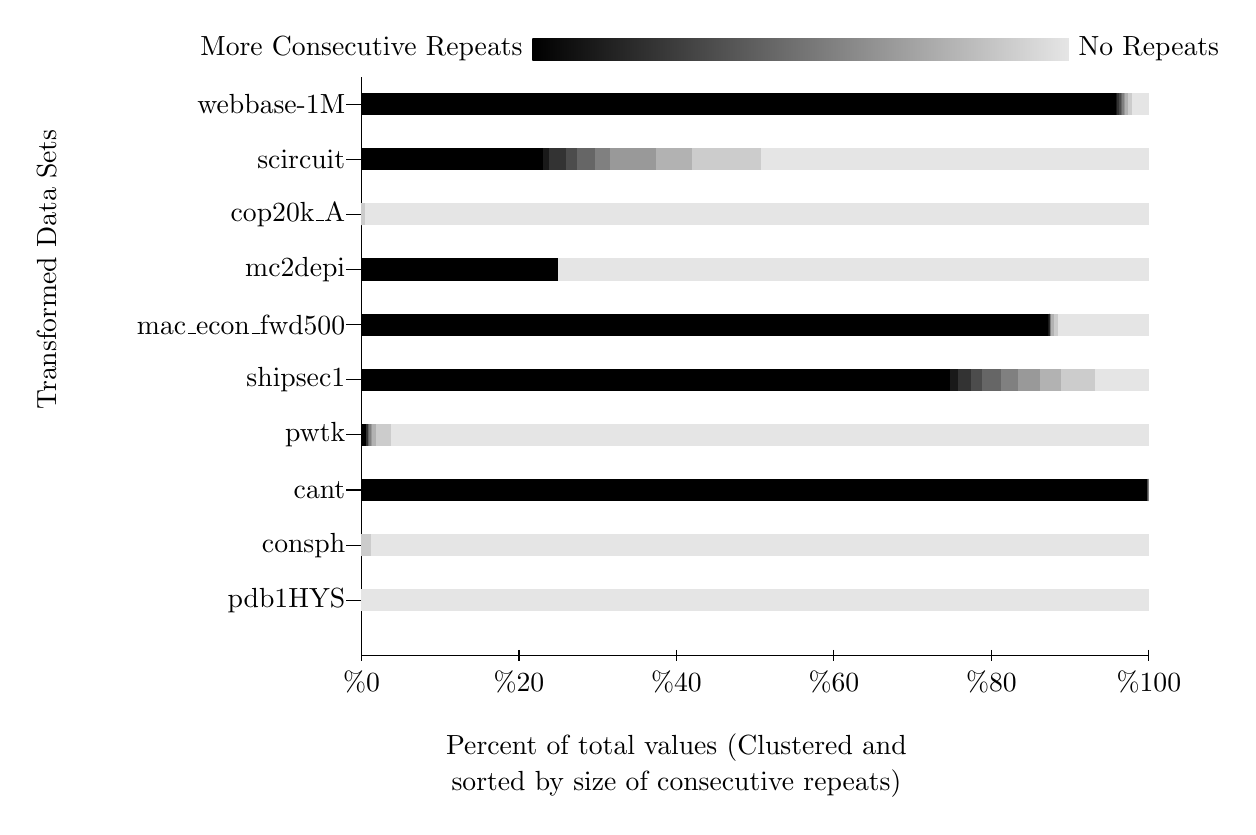
\begin{tikzpicture}[yscale=.7,xscale=2]
\path[draw] (0,0) -- (0,10.5);
\path[draw] (0,0) -- (5,0);
\foreach \x/\v in {0/0,1/20,2/40,3/60,4/80,5/100}{
    \draw (\x,.1) -- (\x,-.1)node[anchor=north]{\%\v};
}
\node[fill=white] at (0,11)(high){More Consecutive Repeats};
\node[fill=white] at (5,11)(low){No Repeats};
\shade[left color=black,right color=black!10] ([yshift=-.2cm]high.east) rectangle ([yshift=.2cm]low.west);

\foreach \n/\y in {pdb1HYS/1, consph/2, cant/3, pwtk/4, shipsec1/5, mac\_econ\_fwd500/6, mc2depi/7, cop20k\_A/8, scircuit/9, webbase-1M/10}{
    \draw (.1,\y) -- (-.1,\y)node[anchor=east,rotate=0,inner sep=0]{\n};
}
\node at (2,-2){\shortstack{Percent of total values (Clustered and \\sorted by size of consecutive repeats)}};
\node[rotate=90] at (-2,7){Transformed Data Sets};

\foreach \s/\xa/\xb in {
100/0.00/0.00,90/0.00/0.00,80/0.00/0.00,70/0.00/0.00,60/0.00/0.00,50/0.00/0.00,40/0.00/0.00,30/0.00/0.00,20/0.00/0.00,10/0.00/5.00}{
    \fill[black!\s] (\xa,0.8) rectangle (\xb,1.2);
}
\foreach \s/\xa/\xb in {
100/0.00/0.00,90/0.00/0.00,80/0.00/0.00,70/0.00/0.00,60/0.00/0.00,50/0.00/0.00,40/0.00/0.00,30/0.00/0.00,20/0.00/0.06,10/0.06/5.00}{
    \fill[black!\s] (\xa,1.8) rectangle (\xb,2.2);
}
\foreach \s/\xa/\xb in {
100/0.00/4.99,90/4.99/4.99,80/4.99/4.99,70/4.99/5.00,60/5.00/5.00,50/5.00/5.00,40/5.00/5.00,30/5.00/5.00,20/5.00/5.00,10/5.00/5.00}{
    \fill[black!\s] (\xa,2.8) rectangle (\xb,3.2);
}
\foreach \s/\xa/\xb in {
100/0.00/0.03,90/0.03/0.03,80/0.03/0.04,70/0.04/0.04,60/0.04/0.05,50/0.05/0.06,40/0.06/0.07,30/0.07/0.09,20/0.09/0.19,10/0.19/5.00}{
    \fill[black!\s] (\xa,3.8) rectangle (\xb,4.2);
}
\foreach \s/\xa/\xb in {
100/0.00/3.74,90/3.74/3.79,80/3.79/3.87,70/3.87/3.94,60/3.94/4.06,50/4.06/4.17,40/4.17/4.31,30/4.31/4.44,20/4.44/4.66,10/4.66/5.00}{
    \fill[black!\s] (\xa,4.8) rectangle (\xb,5.2);
}
\foreach \s/\xa/\xb in {
100/0.00/4.36,90/4.36/4.37,80/4.37/4.37,70/4.37/4.37,60/4.37/4.37,50/4.37/4.38,40/4.38/4.38,30/4.38/4.40,20/4.40/4.42,10/4.42/5.00}{
    \fill[black!\s] (\xa,5.8) rectangle (\xb,6.2);
}
\foreach \s/\xa/\xb in {
100/0.00/1.25,90/1.25/1.25,80/1.25/1.25,70/1.25/1.25,60/1.25/1.25,50/1.25/1.25,40/1.25/1.25,30/1.25/1.25,20/1.25/1.25,10/1.25/5.00}{
    \fill[black!\s] (\xa,6.8) rectangle (\xb,7.2);
}
\foreach \s/\xa/\xb in {
100/0.00/0.00,90/0.00/0.00,80/0.00/0.00,70/0.00/0.00,60/0.00/0.00,50/0.00/0.00,40/0.00/0.00,30/0.00/0.00,20/0.00/0.02,10/0.02/5.00}{
    \fill[black!\s] (\xa,7.8) rectangle (\xb,8.2);
}
\foreach \s/\xa/\xb in {
100/0.00/1.15,90/1.15/1.19,80/1.19/1.30,70/1.30/1.37,60/1.37/1.48,50/1.48/1.58,40/1.58/1.87,30/1.87/2.10,20/2.10/2.54,10/2.54/5.00}{
    \fill[black!\s] (\xa,8.8) rectangle (\xb,9.2);
}
\foreach \s/\xa/\xb in {
100/0.00/4.79,90/4.79/4.80,80/4.80/4.81,70/4.81/4.82,60/4.82/4.83,50/4.83/4.84,40/4.84/4.85,30/4.85/4.87,20/4.87/4.89,10/4.89/5.00}{
    \fill[black!\s] (\xa,9.8) rectangle (\xb,10.2);
}

%TODO: key
\small
%\node at (2,14) {\shortstack{Percent of values in repeating sequences of length $\geq10$ \tikz \draw[fill=green] (0,0) rectangle (.25,.25);,\\ between $10$ and $1$ \tikz \draw[fill=yellow] (0,0) rectangle (.25,.25);, $=1$ \tikz \draw[fill=red] (0,0) rectangle (.25,.25);}};
\end{tikzpicture}
\caption[Floating point pattern analysis using BWT.]{Pattern analysis using the Burrows-Wheeler Transform. Each shade represents the number of consecutive repeats in a repeating sequence. \tikz{\fill[black] (0,0) rectangle (.25,.25);} represents sequences longer than 9. \tikz \fill[black!50] (0,0) rectangle (.25,.25); represents sequences of length 5. \tikz \fill[black!10] (0,0) rectangle (.25,.25); represents sequences equal to 1 (non-repeating).}
\label{fig:pattern}
\end{figure}

\section{Our Approach}
\label{sec:fzipapproach}
Since BWT does not provide great compression, depends on the traversal of the matrix and is not hardware amenable, we designed fzip to only use prefix and repeat compression.
\begin{figure}
\center
\begin{subfigure}{\linewidth}
\center
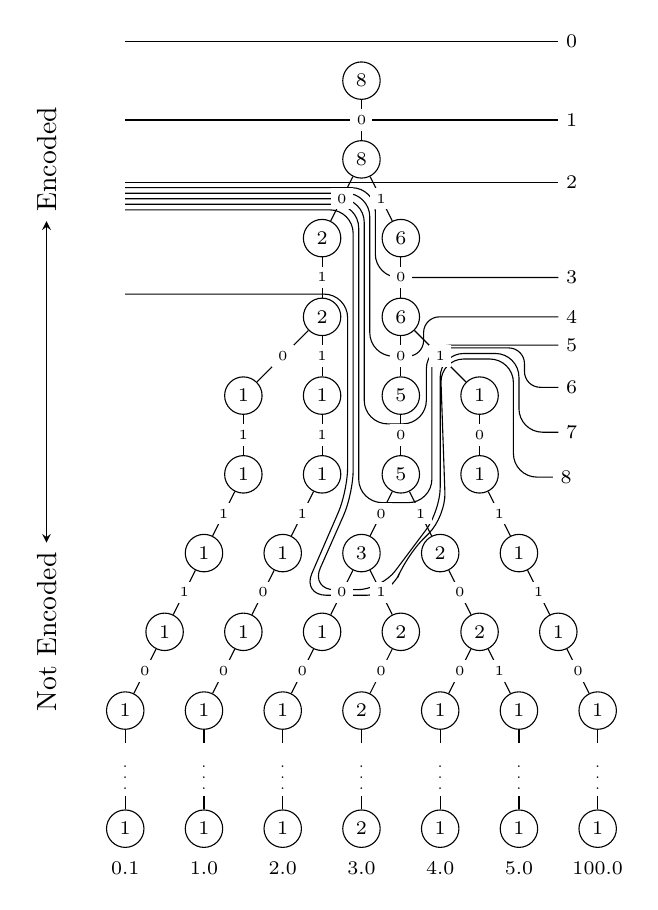
\begin{tikzpicture}
\scriptsize
\node[draw,circle] at (0,0)(n00){8};
%level1
\node[draw,circle] at (0,-1)(n10){8};
%level2
\node[draw,circle] at (-.5,-2)(n20){2};
\node[draw,circle] at (.5,-2)(n21){6};
\node[draw,circle] at (-.5,-3)(n30){2};
\node[draw,circle] at (.5,-3)(n31){6};

\node[draw,circle] at (-1.5,-4)(n40){1};
\node[draw,circle] at (-.5,-4)(n41){1};
\node[draw,circle] at (.5,-4)(n42){5};
\node[draw,circle] at (1.5,-4)(n43){1};

\node[draw,circle] at (-1.5,-5)(n50){1};
\node[draw,circle] at (-.5,-5)(n51){1};
\node[draw,circle] at (.5,-5)(n52){5};
\node[draw,circle] at (1.5,-5)(n53){1};

\node[draw,circle] at (-2,-6)(n60){1};
\node[draw,circle] at (-1,-6)(n61){1};
\node[draw,circle] at (0,-6)(n62){3};
\node[draw,circle] at (1,-6)(n63){2};
\node[draw,circle] at (2,-6)(n64){1};

\node[draw,circle] at (-2.5,-7)(n70){1};
\node[draw,circle] at (-1.5,-7)(n71){1};
\node[draw,circle] at (-0.5,-7)(n72){1};
\node[draw,circle] at (0.5,-7)(n73){2};
\node[draw,circle] at (1.5,-7)(n74){2};
\node[draw,circle] at (2.5,-7)(n75){1};

\node[draw,circle] at (-3,-8)(n80){1};
\node[draw,circle] at (-2,-8)(n81){1};
\node[draw,circle] at (-1, -8)(n82){1};
\node[draw,circle] at (0, -8)(n83){2};
\node[draw,circle] at (1, -8)(n84){1};
\node[draw,circle] at (2, -8)(n85){1};
\node[draw,circle] at (3, -8)(n86){1};

\node[draw,circle] at (-3,-9.5)(n90){1};
\node[draw,circle] at (-2,-9.5)(n91){1};
\node[draw,circle] at (-1,-9.5)(n92){1};
\node[draw,circle] at (0,-9.5)(n93){2};
\node[draw,circle] at (1,-9.5)(n94){1};
\node[draw,circle] at (2,-9.5)(n95){1};
\node[draw,circle] at (3,-9.5)(n96){1};
\scriptsize
\node at (-3,-10){0.1};
\node at (-2,-10){1.0};
\node at (-1,-10){2.0};
\node at (0,-10){3.0};
\node at (1,-10){4.0};
\node at (2,-10){5.0};
\node at (3,-10){100.0};

\scriptsize
\path[draw] (-3,.5) -- (2.5,.5)[anchor=west]node{0};
\path[draw] (-3,-.5) -- (2.5,-.5)[anchor=west]node{1};
\path[draw,yshift=6] (-3,-1.5) -- (2.5,-1.5)[anchor=west]node{2};
%\path[draw,rounded corners=.3cm,yshift=.2cm] (-2.5, -1.5) [shift={(.2cm,.2cm)}] -- (0, -1.5) -- (0,-2.5) -- (2,-2.5);
\path[draw,rounded corners=.3cm,yshift=4] (-3, -1.5) [xshift=5]-- (0, -1.5) [yshift=-4]-- (0,-2.5) [xshift=-5]-- (2.5,-2.5)node[anchor=west]{3};
\path[draw,rounded corners=.3cm,yshift=2] (-3, -1.5) [xshift=3]-- (0, -1.5) [yshift=-2]-- (0,-3.5) [xshift=-9,rounded corners=.2cm] -- (1,-3.5) -- (1,-3) [xshift=6]-- (2.5,-3)node[anchor=west]{4};

\path[draw,rounded corners=.3cm,yshift=0] (-3, -1.5) [xshift=1]-- (0, -1.5) [yshift=4]-- (0,-4.5) [xshift=-6]-- (1,-4.5) -- (1,-3.5) [xshift=5]-- (2.5,-3.5)node[anchor=west]{5};
\path[draw,rounded corners=.3cm,yshift=-2] (-3, -1.5) [xshift=-1]-- (0, -1.5) [yshift=6]-- (0,-5.5) [xshift=-2]-- (1,-5.5) [rounded corners=.2cm,yshift=-1]-- (1,-3.5) [xshift=5]-- (2,-3.5) -- (2,-4) [xshift=-2]-- (2.5,-4)node[anchor=west]{6};
\path[draw,rounded corners=.3cm,yshift=-4] (-3, -1.5) [xshift=-3]-- (0, -1.5) [yshift=-3]-- (0,-5) [shift={(6pt,8pt)}]-- (-.75,-6.5) [xshift=-3]-- (.25,-6.5) -- (1,-5.5) -- (1,-3.5) -- (2,-3.5) -- (2,-4.5) -- (2.5,-4.5)node[anchor=west]{7};
\path[draw,rounded corners=.3cm,yshift=-6] (-3, -2.5) [xshift=-5]-- (0, -2.5) -- (0,-5) [shift={(5pt,5pt)}]-- (-.75,-6.5) [xshift=2]-- (.3,-6.5) -- (.5,-6) -- (1,-5.5) [xshift=-2pt]-- (1,-3.5) [xshift=-2]-- (2,-3.5) -- (2,-5) -- (2.5,-5)node[anchor=west]{8};
%\path[draw,rounded corners=.3cm,yshift=-6] (-3, -1.5) [xshift=-5]-- (0, -1.5) -- (0,-5) [shift={(5pt,5pt)}]-- (-.75,-6.5) -- (0,-6.5) [yshift=1]-- (0,-7.5) [rounded corners=.2cm]-- (1,-7.5) [shift={(2pt,-2pt)}]-- (1,-7) -- (.5,-6) -- (.75,-5.5) [xshift=-2pt]-- (1.5,-5.5) -- (1.5,-6) -- (2,-6)node[anchor=west]{8};

%\path[draw] (-2.5,-8.4) .. controls (-2,-8.4) and (-1.7,-8.3) .. (-1.5,-7.9) -- (0,-5) .. controls (.1,-4.8) and (0,-4.5) .. (1,-4.5) -- (2,-4.5)[anchor=west]node{2};
%\path[draw] (-2.5,-8.5) .. controls (-2,-8.5) and (-1.7,-8.4) .. (-1.5,-8.1) -- (-.2,-5.5) .. controls (0,-5.4) .. (.2,-5.5) -- (.5,-6) .. controls (.8,-6.6) and (.8,-6.5) ..(1.5,-6.5) .. controls (2,-6.5) and (1.5,-5.5) .. (2,-5.5)[anchor=west]node{3};
%\path[draw] (-2.5, -8.6) -- (0,-8.6) .. controls (.1,-8.6) and (.2,-8.6) .. (.5,-8) -- (1,-7) .. controls (1.3,-6.5) and (1,-6.6) ..(2,-6.6)node[anchor=west]{4};
%\path[draw] (-2.5, -8.7) -- (2,-8.7)node[anchor=west]{5};
%\path[draw] (
\tiny
\path[draw] (n00) --node[fill=white]{0} (n10);
\path[draw] (n10) --node[fill=white]{0} (n20);
\path[draw] (n10) --node[fill=white]{1} (n21);
\path[draw] (n20) --node[fill=white]{1} (n30);
\path[draw] (n21) --node[fill=white]{0} (n31);
\path[draw] (n30) --node[fill=white]{0} (n40);
\path[draw] (n30) --node[fill=white]{1} (n41);
\path[draw] (n31) --node[fill=white]{0} (n42);
\path[draw] (n31) --node[fill=white]{1} (n43);

\path[draw] (n40) --node[fill=white]{1} (n50);
\path[draw] (n41) --node[fill=white]{1} (n51);
\path[draw] (n42) --node[fill=white]{0} (n52);
\path[draw] (n43) --node[fill=white]{0} (n53);

\path[draw] (n50) --node[fill=white]{1} (n60);
\path[draw] (n51) --node[fill=white]{1} (n61);
\path[draw] (n52) --node[fill=white]{0} (n62);
\path[draw] (n52) --node[fill=white]{1} (n63);
\path[draw] (n53) --node[fill=white]{1} (n64);

\path[draw] (n60) --node[fill=white]{1} (n70);
\path[draw] (n61) --node[fill=white]{0} (n71);
\path[draw] (n62) --node[fill=white]{0} (n72);
\path[draw] (n62) --node[fill=white]{1} (n73);
\path[draw] (n63) --node[fill=white]{0} (n74);
\path[draw] (n64) --node[fill=white]{1} (n75);

\path[draw] (n70) --node[fill=white]{0} (n80);
\path[draw] (n71) --node[fill=white]{0} (n81);
\path[draw] (n72) --node[fill=white]{0} (n82);
\path[draw] (n73) --node[fill=white]{0} (n83);
\path[draw] (n74) --node[fill=white]{0} (n84);
\path[draw] (n74) --node[fill=white]{1} (n85);
\path[draw] (n75) --node[fill=white]{0} (n86);

\path[draw] (n80) --node[fill=white]{$\vdots$} (n90);
\path[draw] (n81) --node[fill=white]{$\vdots$} (n91);
\path[draw] (n82) --node[fill=white]{$\vdots$} (n92);
\path[draw] (n83) --node[fill=white]{$\vdots$} (n93);
\path[draw] (n84) --node[fill=white]{$\vdots$} (n94);
\path[draw] (n85) --node[fill=white]{$\vdots$} (n95);
\path[draw] (n86) --node[fill=white]{$\vdots$} (n96);

\normalsize
\path (-4,-7)node(ne)[rotate=90]{Not Encoded} -- (-4,-1)node(e)[rotate=90,fill=white]{Encoded};
\path[draw,stealth-stealth] (e)--(ne);
\end{tikzpicture}
\caption{Each node in the above tree represents every prefix that occurs in the dataset.}
\label{fig:tree}
\end{subfigure}
\\
\begin{subfigure}{\linewidth}
\center
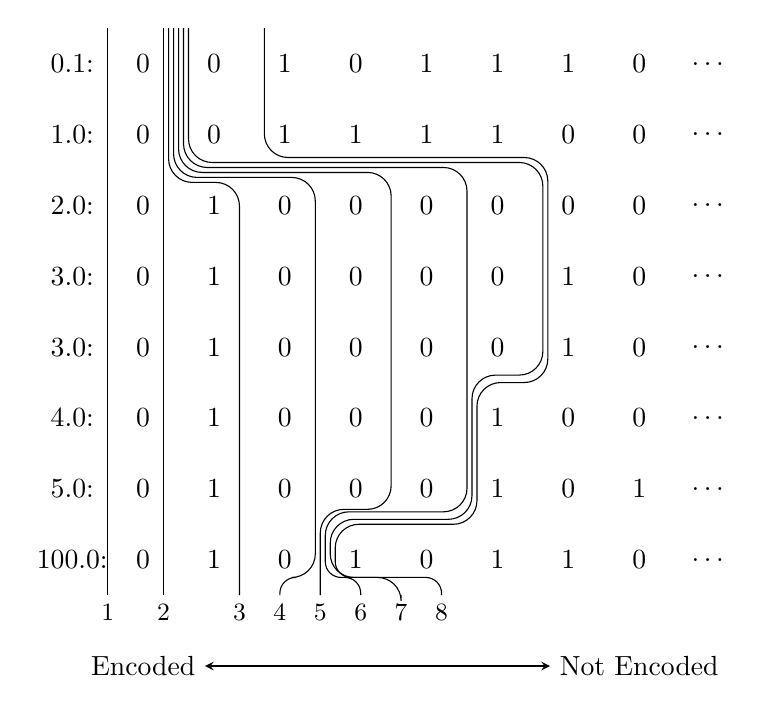
\begin{tikzpicture}[scale=.9]
\node at (0,1){0};\node at (1,1){0};\node at (2,1){1};\node at (3,1){0};\node at (4,1){1};\node at (5,1){1};\node at (6,1){1};\node at (7,1){0};
\node at (0,0){0};\node at (1,0){0};\node at (2,0){1};\node at (3,0){1};\node at (4,0){1};\node at (5,0){1};\node at (6,0){0};\node at (7,0){0};
\node at (0,-1){0};\node at (1,-1){1};\node at (2,-1){0};\node at (3,-1){0};\node at (4,-1){0};\node at (5,-1){0};\node at (6,-1){0};\node at (7,-1){0};
\node at (0,-2){0};\node at (1,-2){1};\node at (2,-2){0};\node at (3,-2){0};\node at (4,-2){0};\node at (5,-2){0};\node at (6,-2){1};\node at (7,-2){0};
\node at (0,-3){0};\node at (1,-3){1};\node at (2,-3){0};\node at (3,-3){0};\node at (4,-3){0};\node at (5,-3){0};\node at (6,-3){1};\node at (7,-3){0};
\node at (0,-4){0};\node at (1,-4){1};\node at (2,-4){0};\node at (3,-4){0};\node at (4,-4){0};\node at (5,-4){1};\node at (6,-4){0};\node at (7,-4){0};
\node at (0,-5){0};\node at (1,-5){1};\node at (2,-5){0};\node at (3,-5){0};\node at (4,-5){0};\node at (5,-5){1};\node at (6,-5){0};\node at (7,-5){1};
\node at (0,-6){0};\node at (1,-6){1};\node at (2,-6){0};\node at (3,-6){1};\node at (4,-6){0};\node at (5,-6){1};\node at (6,-6){1};\node at (7,-6){0};

\node at (8,1){\dots};
\node at (8,0){\dots};
\node at (8,-1){\dots};
\node at (8,-2){\dots};
\node at (8,-3){\dots};
\node at (8,-4){\dots};
\node at (8,-5){\dots};
\node at (8,-6){\dots};

\node at (-1,1){0.1:};\node at (-1,0){1.0:};\node at (-1,-1){2.0:};\node at (-1,-2){3.0:};\node at (-1,-3){3.0:};\node at (-1,-4){4.0:};\node at (-1,-5){5.0:};\node at (-1,-6){100.0:};

\small

\path[draw] (-.5,1.5) -- (-.5,-6.5)node[anchor=north]{1};
\path[draw,xshift=-6] (.5,1.5) -- (.5,-6.5)node[anchor=north]{2};
\path[draw,rounded corners=.3cm,xshift=-4] (.5,1.5) [yshift=-5]-- (.5,-.5) -- (1.5,-.5) [yshift=5]-- (1.5,-6.5)node[anchor=north]{3};
\path[draw,rounded corners=.3cm,xshift=-2] (.5,1.5) [yshift=-3]-- (.5,-.5) -- (2.5,-.5) [yshift=3]-- (2.5,-6.25) [rounded corners=.2cm]-- (2,-6.25) -- (2,-6.5)node[anchor=north]{4};
\path[draw,rounded corners=.3cm,xshift=0] (.5,1.5) [yshift=-1]-- (.5,-.5) -- (3.5,-.5) [yshift=7]-- (3.5,-5.5) -- (2.5,-5.5) [yshift=-6]-- (2.5,-6.5)node[anchor=north]{5};
\path[draw,rounded corners=.3cm,xshift=2] (.5,1.5) [yshift=1]-- (.5,-.5) -- (4.5,-.5) [yshift=4]-- (4.5,-5.5) -- (2.5,-5.5)[rounded corners=.2cm,yshift=-5]-- (2.5,-6.25) -- (3,-6.25) -- (3,-6.5)node[anchor=north]{6};
\path[draw,rounded corners=.3cm,xshift=4] (.5,1.5) [yshift=3]-- (.5,-.5) -- (5.5,-.5) -- (5.5, -3.5) -- (4.5,-3.5) [yshift=-1]-- (4.5,-5.5) -- (2.5,-5.5) [yshift=-2]-- (2.5,-6.25) -- (3.5,-6.25) -- (3.5,-6.5)node[anchor=north]{7};
\path[draw,rounded corners=.3cm,xshift=6] (1.5,1.5) [yshift=5]-- (1.5,-.5) -- (5.5,-.5) [yshift=-5]-- (5.5,-1.5) -- (5.5,-3.5) -- (4.5,-3.5) -- (4.5,-5.5) -- (2.5,-5.5)[rounded corners=.2cm]-- (2.5,-6.25) -- (4,-6.25) -- (4,-6.5)node[anchor=north]{8};
%\path[draw,rounded corners=.3cm,xshift=6] (.5,1.5) [yshift=5]-- (.5,-.5) -- (5.5,-.5) [yshift=-5]-- (5.5,-1.5) -- (6.5,-1.5) -- (6.5, -3.5) -- (4.5,-3.5) [rounded corners=.2cm]-- (4.5,-5.25) -- (5,-5.25) -- (5,-5.5)node[anchor=north]{8};
\normalsize
\path (0,-7.5)node(e){Encoded} -- (7,-7.5)node(ne){Not Encoded};
\path[draw,stealth-stealth] (e)--(ne);
\end{tikzpicture}
\caption{The above sorted list of values gives a second visual representation of how the partition grows.}
\end{subfigure}
\caption[The floating point prefix compression algorithm.]{The above 2 figures show the first 8 partition cuts for prefix compression for the example dataset \{0.1, 1.0, 3.0, 5.0, 3.0, 100.0, 4.0, 2.0\}. For simplicity half-precision (16-bit) encoding is used.}
\label{fig:jiles}
\end{figure}
\subsection{Prefix Compression}
fzip uses arithmetic encoding followed by Huffman encoding to encode common prefixes. To begin with, fzip creates a large tree to represent all the values in the array. \figurename~\ref{fig:tree} shows an example tree for a small dataset. The tree follows the following rules: each node has up to two children. Each edge represents a 1 bit or a 0 bit. Each node in the tree represents a prefix. The root node represents ``" or no prefix. Each node also has a weight, which represents the number of values with the prefix the node represents. So, the weight of the root node equals the total number of values. The weight of the left (or 0 bit) child of the root represents the prefix ``0". Its weight represents the number of  values that start with ``0" (all non-negative values). Likewise, the right child of the root represents the prefix ``1" and its weight is the number of values starting with 1 (all the negative values).\par
Several properties appear. First, the sum of all the weights of the nodes in any level equals $nnz$, where $nnz$ is the total number of values. Moreover, the weight of any set of nodes that partitions the root node from the $65^{th}$ level (and does not contain more nodes than necessary to create the partition) equals $nnz$.\par
Second, the tree is unbalanced (in our case this is good). Put another way, the datasets contain an unequal number of positive and negative numbers, also any ``normal" dataset would not have an exponential distribution from $2^{-12}$ to $2^{12}$ in such a way to make the rest of the tree balanced.\par
Tree creation starts with the root node, which has a starting weight of 0. To create the rest of the tree, add each value to the tree in the following way: Create a pointer to a ``current node" $c$ and initiate $c$ to the root node. Increment the weight of $c$ (the root node). Then, with the most significant bit (the sign bit) of the floating point value, update $c$ by following the edge that matches this bit. If this edge does not exist create the edge and corresponding node. Then, increment the weight of the new $c$. This repeats until you reach the $64^{th}$ bit. Then, the next value gets added to the tree. This continues until the last value gets added to the tree.\par
fzip calculates the prefix codes by creating a partition in the tree. To start, fzip creates a partition with only the root node. Then it includes the node with the largest weight that is a child of the partition. This repeats until a predetermined number of edges become cut by the partition. Using a list of prefix, prefix code pairs we can represent the encoding scheme of the first 8 partitions of the example in \figurename~\ref{fig:jiles}:\par
\begin{enumerate}
    \item (0,)
    \item (00,0), (01,1)
    \item (00,0), (010,1)
    \item (00,00), (0100,01), (0101,10)
    \item (00,00), (01000,01), (0101,10)
    \item (00,00), (010000,01), (010001,10), (0101,11)
    \item (00,000), (0100000,001), (0100001,010), (010001,011), (0101,100)
    \item (001,000), (0100000,001), (0100001,010), (010001,011), (0101,100)
\end{enumerate} \par
Each added node improves the compression because of the following observation: Let the last added node equal $A$. The number of bits in the uncompressed (not-encoded) stream decreases by weight($A$). However, the code lengths have to increase because the partition cut-size ($k$) increases. The code lengths equal $\log_2(k)$. So the increase in the code length equals $\log_2(k+1)-\log_2(k)$ or $\frac{1}{k}$ by using derivatives. So the codes stream will increase by $\frac{nnz}{k}$, where $nnz$ equals to number of values in the data set. If you choose $A$ to maximize $\textrm{weight}(A)$ (a greedy algorithm) then $\textrm{weight}(A) > \textrm{average weight of children to the partition} = \frac{nnz}{k}$. Therefore, the total size of the prefix compression, excluding overhead, keeps improving as the partition increases.\\
\indent But, what if a value occurs often? Say the value $1.0$ occurs $10\%$ of the time? Ideally you should encode $1.0$ as 4 bits ($\log_210$ rounded up), but if we continue to grow the partition beyond cutting 16 edges $1.0$ would encode as more than 4 bits. Our solution freezes the codes once a node from the last ($65^{th}$) level becomes included in the partition. This allows fzip to continue to improve prefix compression by growing the partition and also encode common values with shorter codes. This change makes the encoding to variable-length arithmetic encoding.\\
\indent Of course, the overhead to store all of the codes exists. Currently, a 16 byte record describes each code. Each record stores the prefix, the prefix length and the code length. To balance the benefit of prefix encoding with its overhead, we limit the overhead to 256 records.
\subsection{Repeated Value Extension}
Prefix compression does not compress all of the repeated values. So, fzip extends prefix compression to specifically include commonly repeated values. Again explaining why repeated values compress well: All of the datasets have less than 6 million values. An index of 23 bits can address the entire dataset. Even if a value repeats only once (occurs twice) there still exists an advantage to store the repeated values in a repeated value array and store the indexes into this array instead of the original values. In the previous example $23+23+64<64+64$ (2 indices plus the value in the array equals less than storing 2 values).\\
\indent To encode these repeats, we add a special code to the set of prefix codes. We limit the number of repeats to 8192, so when this code is encountered 13 bits will be on the not-encoded stream indicating the address of the common value.

\begin{figure}
\center
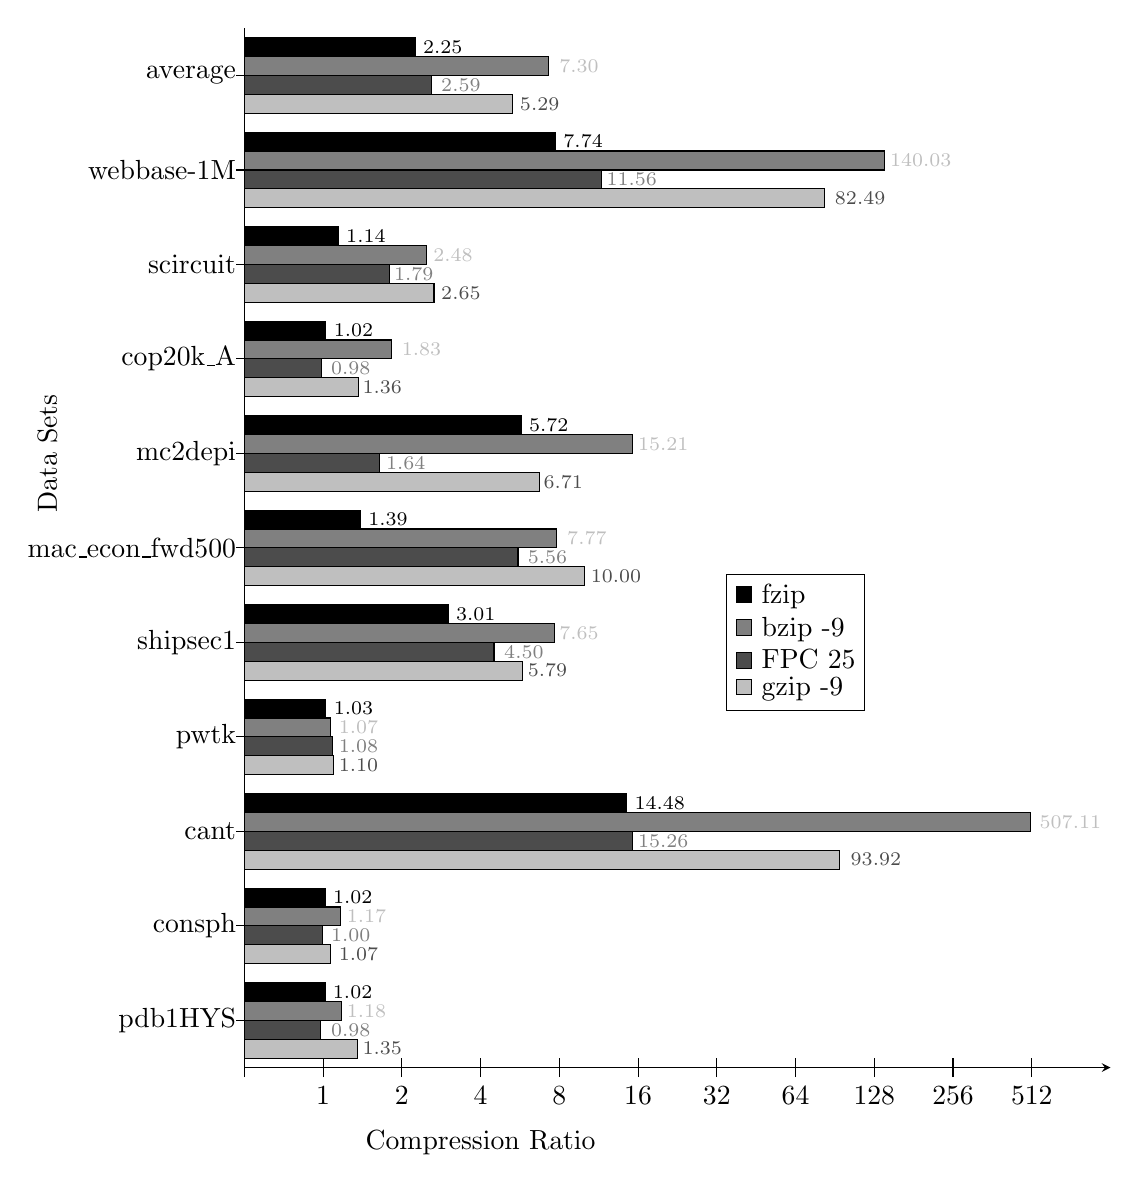
\begin{tikzpicture}[xscale=1,yscale=1.2]
\path[draw] (0,.5) -- (0,11.5);
\path[draw, -stealth] (0,.5) -- (11,.5);
\foreach \x in {0,1,...,10}{
    \path[draw](\x,.4) -- (\x,.6);
}
\foreach \n/\y in {pdb1HYS/1, consph/2, cant/3, pwtk/4, shipsec1/5, mac\_econ\_fwd500/6, mc2depi/7, cop20k\_A/8, scircuit/9, webbase-1M/10, average/11}{
    \draw (.1,\y) -- (-.1,\y)node[anchor=east,rotate=0,inner sep=0]{\n};
}
\foreach \x/\xscale in {1/1,2/2,3/4,4/8,5/16,6/32,7/64,8/128,9/256,10/512}{
    \node[anchor=north] at (\x,.4){\xscale};
}
%labels
\node[rotate = 90] at (-2.5,7){Data Sets};
\node at (3, -.3){Compression Ratio};
%TODO: data
%black!50 black!25 black!70 yellow
%gzip
\foreach \y/\val in
{
    1/1.4381395476381393,2/1.0916733147798856,3/7.553384991365857,4/1.134840892559168,5/3.5325464816899257,6/4.3220742537498005,7/3.7452968046629334,8/1.4474437031978624,9/2.4082861931969743,10/7.3662162703581915,11/3.4039902453198736
}{
    \draw[fill=black!25] (0,\y-.4) rectangle (\val,\y-.2);
}

\foreach \y/\val in {
1/0.9703154387982447,2/0.9940709630537352,3/4.9313813811158385,4/1.1162887682756681,5/3.170250966398405,6/3.475248978449822,7/1.7113132878531525,8/0.9757434397200309,9/1.8431713715699232,10/4.530812321248466,11/2.371859691648329
}{
    \draw[fill=black!70] (0,\y-.2) rectangle (\val,\y);
}


\foreach \y/\val in
{
1/1.2342280655474396,2/1.2260093429943355,3/9.986162958869974,4/1.0951017190297625,5/3.93629964487195,6/3.9586175034412285,7/4.926834410237387,8/1.8710214839874202,9/2.3088144122961687,10/8.12964239568333,11/3.8672731936958997
}{
    \draw[fill=black!50] (0,\y) rectangle (\val,\y+.2);
}

\foreach \y/\val in {
%1/1.182412629081373,2/1.204366120271175,3/5.3579179101253285,4/1.1414066312172233,5/3.959223014150452,6/3.8767389203500864,7/3.648371101032564,8/1.2800298418189981,9/2.252300597334877,10/6.4002885786378085,11/3.0303055344019887
1/1.0247843066796307,2/1.0253806882643661,3/4.855947836037533,4/1.0356772378945645,5/2.588433170987532,6/1.4737000206741608,7/3.515524876460967,8/1.0350216323270796,9/1.1932676349618145,10/3.9521755145314765,11/2.169991291881913
}{
    \draw[fill=black] (0,\y+.2) rectangle (\val,\y+.4);
}


\scriptsize
\node[black,anchor=west] at (1.0247843066796307,1.3){1.02};
\node[black,anchor=west] at (1.0253806882643661,2.3){1.02};
\node[black,anchor=west] at (4.855947836037533,3.3){14.48};
\node[black,anchor=west] at (1.0356772378945645,4.3){1.03};
\node[black,anchor=west] at (2.588433170987532,5.3){3.01};
\node[black,anchor=west] at (1.4737000206741608,6.3){1.39};
\node[black,anchor=west] at (3.515524876460967,7.3){5.72};
\node[black,anchor=west] at (1.0350216323270796,8.3){1.02};
\node[black,anchor=west] at (1.1932676349618145,9.3){1.14};
\node[black,anchor=west] at (3.9521755145314765,10.3){7.74};
\node[black,anchor=west] at (2.169991291881913,11.3){2.25};

\node[black!50,anchor=west] at (1.0,0.9){0.98};
%\node[black,anchor=west] at (1.2,1.3){1.13};
\node[black!25,anchor=west] at (1.2,1.1){1.18};
\node[black!70,anchor=west] at (1.4,0.7){1.35};
\node[black!50,anchor=west] at (1.0,1.9){1.00};
\node[black!70,anchor=west] at (1.1,1.7){1.07};
%\node[black,anchor=west] at (1.2,2.3){1.15};
\node[black!25,anchor=west] at (1.2,2.1){1.17};
\node[black!50,anchor=west] at (4.9,2.9){15.26};
%\node[black,anchor=west] at (5.4,3.3){20.51};
\node[black!70,anchor=west] at (7.6,2.7){93.92};
\node[black!25,anchor=west] at (10.0,3.1){507.11};
\node[black!25,anchor=west] at (1.1,4.1){1.07};
\node[black!50,anchor=west] at (1.1,3.9){1.08};
\node[black!70,anchor=west] at (1.1,3.7){1.10};
%\node[black,anchor=west] at (1.1,4.3){1.10};
\node[black!50,anchor=west] at (3.2,4.9){4.50};
\node[black!70,anchor=west] at (3.5,4.7){5.79};
\node[black!25,anchor=west] at (3.9,5.1){7.65};
%\node[black,anchor=west] at (4.0,5.3){7.78};
\node[black!50,anchor=west] at (3.5,5.9){5.56};
%\node[black,anchor=west] at (3.9,6.3){7.34};
\node[black!25,anchor=west] at (4.0,6.1){7.77};
\node[black!70,anchor=west] at (4.3,5.7){10.00};
\node[black!50,anchor=west] at (1.7,6.9){1.64};
%\node[black,anchor=west] at (3.6,7.3){6.27};
\node[black!70,anchor=west] at (3.7,6.7){6.71};
\node[black!25,anchor=west] at (4.9,7.1){15.21};
\node[black!50,anchor=west] at (1.0,7.9){0.98};
%\node[black,anchor=west] at (1.3,8.3){1.21};
\node[black!70,anchor=west] at (1.4,7.7){1.36};
\node[black!25,anchor=west] at (1.9,8.1){1.83};
\node[black!50,anchor=west] at (1.8,8.9){1.79};
%\node[black,anchor=west] at (2.3,9.3){2.38};
\node[black!25,anchor=west] at (2.3,9.1){2.48};
\node[black!70,anchor=west] at (2.4,8.7){2.65};
\node[black!50,anchor=west] at (4.5,9.9){11.56};
%\node[black,anchor=west] at (6.4,10.3){42.23};
\node[black!70,anchor=west] at (7.4,9.7){82.49};
\node[black!25,anchor=west] at (8.1,10.1){140.03};
\node[black!50,anchor=west] at (2.4,10.9){2.59};
%\node[black,anchor=west] at (3.0,11.3){4.08};
\node[black!70,anchor=west] at (3.4,10.7){5.29};
\node[black!25,anchor=west] at (3.9,11.1){7.30};
%\node[black!50,anchor=west] at (1.1,1.1){1.09};
%\node[black,anchor=west] at (1.2,1.3){1.12};
%\node[black!25,anchor=west] at (1.2,0.7){1.13};
%\node[black!70,anchor=west] at (1.4,0.9){1.29};
%\node[black!50,anchor=west] at (1.0,2.1){1.02};
%\node[black!25,anchor=west] at (1.1,1.7){1.05};
%\node[black,anchor=west] at (1.1,2.3){1.08};

\normalsize
\node[draw] at (7,5){\shortstack[l]{
    \tikz \draw[fill=black] (.1,.1) rectangle (.3,.3); fzip\\
    \tikz \draw[fill=black!50] (.1,.1) rectangle (.3,.3); bzip -9\\
    \tikz \draw[fill=black!70] (.1,.1) rectangle (.3,.3); FPC 25\\
    \tikz \draw[fill=black!25] (.1,.1) rectangle (.3,.3); gzip -9
    }};

\end{tikzpicture}
\caption[Floating point compression comparing gzip, bzip, FPC and fzip.]{The comparison of different compression schemes shows fzip performs competitively.}
\label{fig:compare}
\end{figure}
%\begin{figure}
%\center
%\begin{tikzpicture}[xscale=3, yscale=1.2]
%\path[draw, -stealth] (0,.5) -- (3.5,.5);
%\path[draw] (0,.5) -- (0,14.5);
%\foreach \x in {0,1,...,3}{
%    \path[draw](\x,.6) -- (\x,.4);
%}
%\foreach \n/\y in {dense2/1, pdb1HYS/2, consph/3, cant/4, pwtk/5, rma10/6, qcd5\_4/7, shipsec1/8, mac\_econ\_fwd500/9, mc2depi/10, cop20k\_A/11, scircuit/12, webbase-1M/13, average/14}{
%    \draw (.1,\y) -- (-.1,\y)node[anchor=east,rotate=0,inner sep=0]{\n};
%}
%\foreach \x/\yscale in {1/10K,2/100K,3/1M}{ %,4/10M}{
%    \node[anchor=north] at (\x,.4){\yscale};
%}
%
%\node[rotate=90] at (-1.2,5.5) {Data Sets};
%\node at (2,-.3) {Compressed Values per Second};
%
%\foreach \y/\x in {1/3.34,2/3.48,3/3.31,4/3.30,5/3.00,6/2.15,7/2.37,8/3.13,9/2.03,10/3.49,11/3.18}{
%    \draw[rectangle,fill=black!25] (0,\y-.4) rectangle (\x,\y-.2);
%}
%\foreach \y/\x in {1/3.34,2/1.58,3/3.31,4/3.77,5/0.22,6/2.15,7/2.18,8/3.13,9/2.03,10/2.02,11/3.08}{
%    \draw[rectangle,fill=black!70] (0,\y-.2) rectangle (\x,\y);
%}
%\foreach \y/\x in {1/2.86,2/2.88,3/2.46,4/2.99,5/3.60,6/2.50,7/3.32,8/3.13,9/2.98,10/2.71,11/3.08}{
%    \draw[fill=black!50] (0,\y) rectangle (\x,\y+.2);
%}
%\foreach \y/\x in {1/1.55,2/1.58,3/1.83,4/1.41,5/0.22,6/2.15,7/2.18,8/1.75,9/2.03,10/2.02,11/1.86}{
%    \draw[fill=black] (0,\y+.2) rectangle (\x,\y+.4);
%}
%\scriptsize
%\node[black,anchor=west] at (1.5,1.3){35K};
%\node[black!50,anchor=west] at (2.9,1.1){730K};
%\node[black!25,anchor=west] at (3.3,0.7){2.2M};
%\node[black!70,anchor=west] at (3.3,0.9){2.2M};
%\node[black!70,anchor=west] at (1.6,1.9){38K};
%\node[black,anchor=west] at (1.6,2.3){38K};
%\node[black!50,anchor=west] at (2.9,2.1){762K};
%\node[black!25,anchor=west] at (3.5,1.7){3.0M};
%\node[black,anchor=west] at (1.8,3.3){68K};
%\node[black!50,anchor=west] at (2.5,3.1){291K};
%\node[black!25,anchor=west] at (3.3,2.7){2.0M};
%\node[black!70,anchor=west] at (3.3,2.9){2.0M};
%\node[black,anchor=west] at (1.4,4.3){26K};
%\node[black!50,anchor=west] at (3.0,4.1){988K};
%\node[black!25,anchor=west] at (3.3,3.7){2.0M};
%\node[black!70,anchor=west] at (3.8,3.9){5.9M};
%\node[black!70,anchor=west] at (0.2,4.9){2K};
%\node[black,anchor=west] at (0.2,5.3){2K};
%\node[black!25,anchor=west] at (3.0,4.7){994K};
%\node[black!50,anchor=west] at (3.6,5.1){4.0M};
%\node[black!25,anchor=west] at (2.2,5.7){141K};
%\node[black!70,anchor=west] at (2.2,5.9){141K};
%\node[black,anchor=west] at (2.2,6.3){141K};
%\node[black!50,anchor=west] at (2.5,6.1){318K};
%\node[black!70,anchor=west] at (2.2,6.9){150K};
%\node[black,anchor=west] at (2.2,7.3){150K};
%\node[black!25,anchor=west] at (2.4,6.7){233K};
%\node[black!50,anchor=west] at (3.3,7.1){2.1M};
%\node[black,anchor=west] at (1.8,8.3){57K};
%\node[black!25,anchor=west] at (3.1,7.7){1.4M};
%\node[black!70,anchor=west] at (3.1,7.9){1.4M};
%\node[black!50,anchor=west] at (3.1,8.1){1.4M};
%\node[black!25,anchor=west] at (2.0,8.7){107K};
%\node[black!70,anchor=west] at (2.0,8.9){107K};
%\node[black,anchor=west] at (2.0,9.3){107K};
%\node[black!50,anchor=west] at (3.0,9.1){959K};
%\node[black!70,anchor=west] at (2.0,9.9){104K};
%\node[black,anchor=west] at (2.0,10.3){104K};
%\node[black!50,anchor=west] at (2.7,10.1){518K};
%\node[black!25,anchor=west] at (3.5,9.7){3.1M};
%\node[black,anchor=west] at (1.9,11.3){73K};
%\node[black!50,anchor=west] at (3.1,11.1){1.2M};
%\node[black!70,anchor=west] at (3.1,10.9){1.2M};
%\node[black!25,anchor=west] at (3.2,10.7){1.5M};
%\normalsize
%\node[draw,rotate=90] at (-1.2,10){\tikz \draw[fill=black!25] (.1,.1) rectangle (.3,.3); gzip -9 \tikz \draw[fill=black!70] (.1,.1) rectangle (.3,.3); FPC 25 \tikz \draw[fill=black!50] (.1,.1) rectangle (.3,.3); bzip -9 \tikz \draw[fill=black] (.1,.1) rectangle (.3,.3); fzip};
%\end{tikzpicture}
%\caption{The above compression runtime analysis shows that fzip has some improvement to make to compete with other program's runtime.}
%\label{fig:runtime}
%\end{figure}

\section{The fzip decoder}
\label{sec:fzip_decoder}
Like the SMC decoder from Section~\ref{sec:smc_decoder} in the previous chapter, the fzip hardware decoder relies on lookup tables to decode the two streams (see \figurename~\ref{fig:fzip_decoder}). First the dictionary is loaded onto a large 512 value lookup table (LUT). This lookup table uses the code length to determine how much to shift the first shift buffer. The LUT then determines if the second shift buffer is needed (the code is a variable length delta). Then the delta (or newline) is sent to the running row and column index and the current row and column index is outputted from the decoder.
\begin{figure}
    \begin{tikzpicture}
        \node at (0,1) {Memory};
        \node at (4,1) {Decoder};
        \draw [dashed](1.8,1.5) -- (1.8,-5);
        \node at (-.2,0)[draw,trapezium,trapezium right angle=120,trapezium left angle=60](h){Header};
        \node at (-.2,-1)[draw,trapezium,trapezium right angle=120,trapezium left angle=60](d){Dictionary};
        \node at (-.2,-2)[draw,trapezium,trapezium right angle=120,trapezium left angle=60](common){Commons};
        \node at (-.2,-3.2)[draw,trapezium,trapezium right angle=120,trapezium left angle=60](ds){\shortstack{Data\\Stream}};
        \node at (-.2,-4.6)[draw,trapezium,trapezium right angle=120,trapezium left angle=60](as){\shortstack{Argument\\Stream}};

        \node at (5, 0) [draw,minimum width=4cm](sb1){Shifter Buffer};
        \node at (3.5, -1.5) [draw,minimum height=1cm](l){LUT};
        \node at (5, -3) [draw,minimum width=4cm](sb2){Shifter Buffer};

        \node at (9, -4) [minimum width=2cm](shared){\shortstack{Shared\\Memory}};
        \draw (shared.south west) -- (shared.north west) -- (shared.north east) -- (shared.south east);

        \node at (11,-1.5) (output){Output};

        \draw[->,shorten >=2pt] (ds) .. controls ++(1.5,0)  and ++(-2.5,0) .. (sb1);
        \draw[->,shorten >=2pt] (sb1.350) .. controls ++(0,-.5) and ++(0,.5) .. (l.north -| 3.7,0);
        \draw[<-,shorten <=2pt] (sb1.south -| 3.5,0) .. controls ++(0,-.5) and ++(0,.5) .. (l.north -| 3.3,0);
        \draw[->,shorten >=2pt] (as) .. controls ++(1.5,0) and ++(-2.5,0) .. (sb2);
        \draw[->,shorten >=2pt] (l) -- (l|-sb2.north);
        %\draw (l) |- (sb2);
        \draw[->,shorten >=2pt] (sb2.10) .. controls ++(0,.5) and ++(0,1) .. (shared.north -| 8.8,0);
        \draw[->,shorten >=2pt] (sb2.10) .. controls ++(0,.5) and ++(-1,0) .. (8,-1.5);
        \draw[->,shorten >=2pt] (shared.north -| 9.2,0) .. controls ++(0,1) and ++(-1,0) .. (10,-1.5);
        \draw[->,shorten >=2pt] (d) .. controls ++(1.5,0) and ++(-1,0) .. (l);
        \draw[->,shorten >=2pt] (l) -- (output);

        \draw[->,shorten >=2pt] (common) .. controls ++(3,0) and (0,-4) .. (shared);

    \end{tikzpicture}
    \caption{The hardware design of the fzip decoder.}
    \label{fig:fzip_decoder}
\end{figure}

We do not have the exact area and performance of this decoder because we only designed a decoder that combined the index and floating point decoding. However, the first shift buffer uses 293 LUTs and 60 registers. The second shift buffer uses 957 LUTs and 146 registers. The combined decoder has a top frequency of 150 Mhz after place and route using xst.
\section{Results}
\label{sec:fzipdiscussion}
We present fzip's results in \figurename~\ref{fig:compare}. As seen fzip does not perform quite as well as its competitors. However, fzip is very limited in what it uses for memory space when decompressing. Increasing the common values space from 64KB to an `unlimited' space and increasing the number of prefix codes does increase the compression ratio, but this no longer makes it possible to create a hardware decoder. As the next chapter shows creating an efficient 64KB shared memory on an FPGA is not a trivial task.
